% !Mode:: "TeX:UTF-8"
%!TEX program  = xelatex

%\documentclass{cumcmthesis}
\documentclass[withoutpreface,bwprint]{cumcmthesis} %去掉封面与编号页
\bibliographystyle{unsrt}
\usepackage{subfigure}	%用于排版多张图片
\usepackage{float}	%用于排版图片位置
\usepackage{multirow}
\usepackage{array}
\usepackage{booktabs}
\usepackage{adjustbox}
\bibliographystyle{plain}	%引用样式,参考文献

\usepackage{url}
\title{“板凳龙”运动模型}

\begin{document}
	
	\maketitle
	\begin{abstract}
	%	板凳龙是浙闽地区独具特色的传统民俗活动,是我国非物质文化遗产的重要组成部分。本文通过建立数学模型,研究舞龙队盘入和调头盘出过程中的运动状态和路径优化,为此传统表演提供科学的理论支撑,确保舞龙队的安全,提高表演的观赏性。
		
	本文针对舞龙队沿等距螺线运动的计算问题,从分析龙头的运动状态出发,龙头的位置状态可由旋转角确定且龙头速度恒定,分别求解后续节点的位置和速度。在螺距一定时,考虑舞龙队沿螺线运动,求解舞龙队的终止时刻与此时的运动状态。在舞龙队沿圆弧调头曲线调头和盘出时,求解出调头曲线的最短长度和任意时刻舞龙队的运动状态信息。
	
	针对问题一,对龙头的位置状态进行分析,由龙头所在曲线的极坐标方程和角速度的微分形式建立龙头旋转角度随时间变化的函数关系,并根据余弦定理构建相邻节点的位置递推关系。在求解舞龙队位置时,使用\textbf{牛顿迭代法}来求解余弦定理所构建关系的数值解。对龙头的速度状态进行分析,龙头以恒定速度沿螺线运动,基于位于同一板上两点沿板方向速度分量相等的物理关系构建相邻节点的速度递推关系。通过递推和牛顿迭代的方法求解出从初始时刻到 300 s 为止,每秒整个舞龙队的位置和速度,结果保存在文件result1.xlsx中。
	
	针对问题二,由几何关系求解出舞龙队各节矩形板凳的四个定点坐标,通过遍历判断每节板凳的顶点是否会落入非相邻板凳区域内来确定是否发生碰撞,当恰好发生碰撞时确定此时刻为终止时刻,通过代入问题一建立的舞龙队运动模型得到此时舞龙队的位置和速度,结果保存在result2.xlsx中。
	
	针对问题三,使用龙头前把手到原点的距离来判断龙头是否顺利盘入了调头空间,通过改变螺距根据问题二建立的碰撞模型选择终止时刻龙头的位置来决策。当在调头空间边界恰好发生碰撞时,此时螺距达到最小。在求解最小螺距模型时,使用\textbf{二分法}的思想和\textbf{变步长搜索算法}来寻找最优解,通过计算解得螺距最小取值为\textbf{0.451m}。
	
	针对问题四,对于第一小问,调头曲线的长度仅由盘入点坐标限制,通过建立几何关系可以求解两段圆弧的半径和圆心角,初始时刻调头空间的半径为4.5m通过代入模型可解得此时调头曲线的长度为\textbf{14.854167m},对于模型求解,使用二分法得到最小调头半径为\textbf{2.89m},此时调头曲线长度为\textbf{9.879203m}。对于第二小问,将舞龙队的运动状态分为三类:盘入曲线、调头曲线、盘出曲线,并通过临界旋转角和在调头曲线上的运动时间判断临界点,计算时先判断每节板凳所在曲线,然后代入运动模型求解以调头时刻开始为零时刻,从-100s到100s每秒舞龙队的位置和速度,结果保存在result4.xlsx中。
	
	针对问题五,根据问题四,可以推测当整个舞龙队都进入盘出曲线时,龙尾的速度即为舞龙队中最大的速度。使用二分法求解龙头速度不同时的龙尾速度,找到最大速度刚好小于2m/s时龙头的速度,通过计算解得龙头的最大速度为\textbf{1.989837m/s};
	
	最后在问题三的基础上探究了调头空间圆半径对最小螺距的影响,分析了模型优缺点并提出了改进方向。
		
		\vspace{0.1cm} 
		\noindent \textbf{关键词:等距螺线\quad 牛顿迭代法\quad 二分法\quad 变步长搜索算法\quad }
		
	\end{abstract}
	\vspace{-1.4cm} 
	\section{问题重述}
	\subsection{问题背景}
	“板凳龙”,即“盘龙”,是由众多条板凳首尾相连形成的舞龙,流行于浙闽地区,是我国非遗的重要组成部分。一条舞动千年的情感纽带,承载着中华民族深厚的文化底蕴和民间智慧。盘龙过程中,龙头引领龙身龙尾,盘绕呈圆盘形态。在保证舞龙队可灵活盘入和盘出的前提下,缩小盘龙所需的面积、加快盘龙行进速度是提高观赏性的关键。
	\subsection{问题提出}
	本题中板凳龙由1节龙头,221节龙身,1节龙尾,共223节板凳组成,把手穿过每节板凳上的两个孔连接相邻的两条板凳。已知龙头、龙身和龙尾的板长和板宽,每节板凳两孔的孔径,孔心与邻近板头的长度。
	\begin{figure}[H]
		\centering
		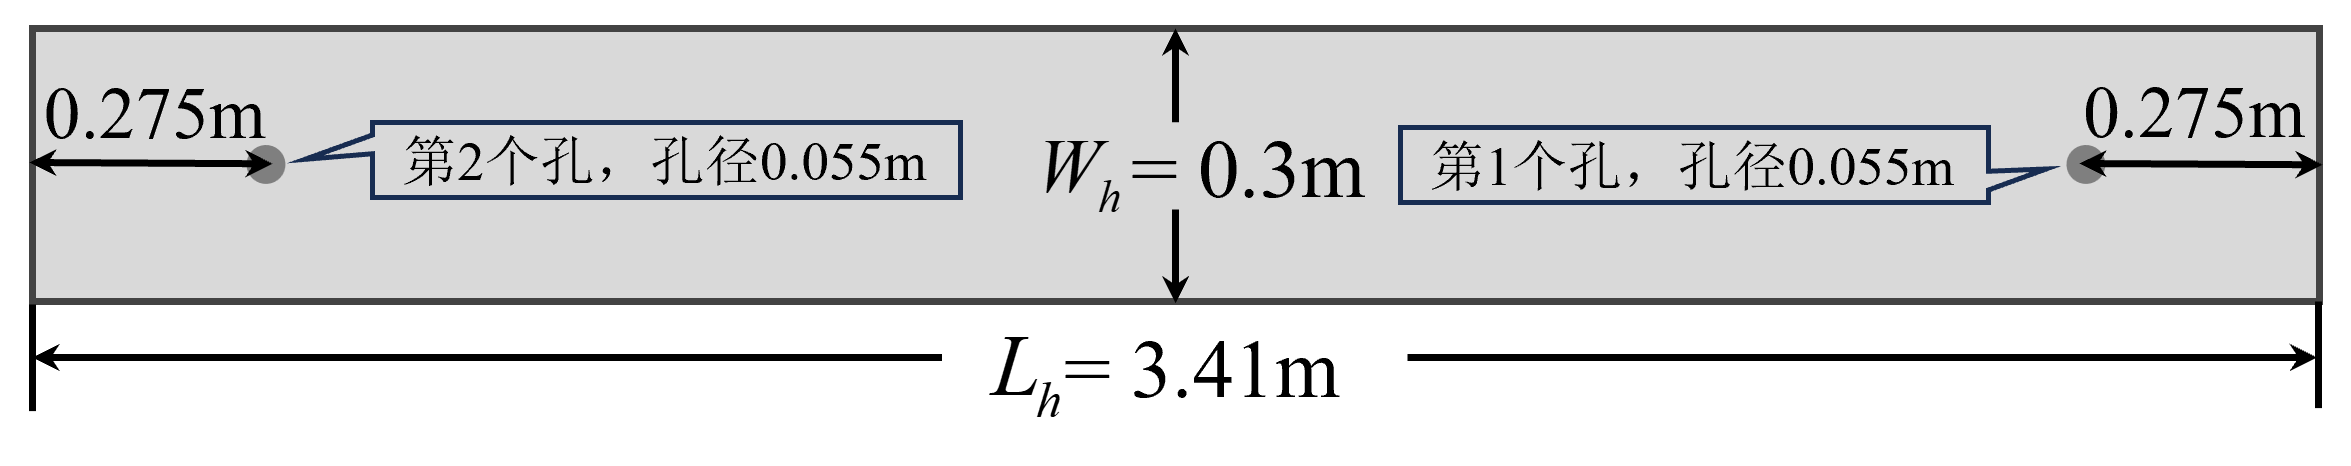
\includegraphics[scale=0.65]{龙头.png}
		\caption{龙头的俯视图}
		%\label{龙头} %在标题之下
	\end{figure}
	\vspace{-0.4cm} 
	\begin{figure}[H]
		\centering
		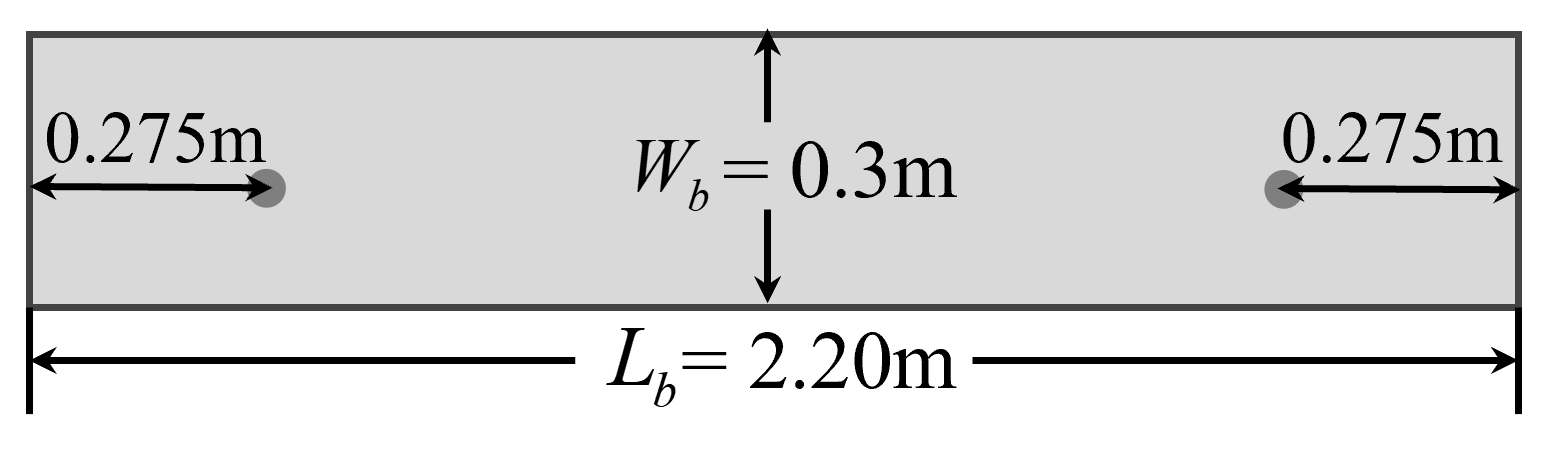
\includegraphics[scale=0.65]{龙身和龙尾.png}
		\caption{龙身和龙尾的俯视图}
		%\label{龙身和龙尾} %在标题之下
	\end{figure}
	基于以上信息,本文建立数学模型解决以下问题:
	
	问题一:考虑舞龙队按照螺距为55cm的等距螺线顺时针盘入。已知起始时刻龙头位置,行进时每个把手的中心均位于螺线上,龙头前把手的行进速度恒定为1m/s。计算从起始时刻到300s时,每秒整个舞龙队各部分的位置和速度,将结果按指定格式保存于文件result1.xlsx中,并给出0 s、 60 s、 120 s、 180 s、 240 s、 300 s 时, 龙头前把手、 龙头后第 1、51、 101、 151、 201节龙身前把手和龙尾后把手的位置和速度。
	
	问题二:在问题一中舞龙队盘入设定的基础上,考虑板凳间不发生碰撞,求解舞龙队停止盘入的时刻,计算此时刻舞龙队各部分的位置和速度,将结果按指定格式保存于文件result2.xlsx中,并给出龙头前把手、 龙头后第 1、51、 101、 151、 201节龙身前把手和龙尾后把手的位置和速度。
	
	问题三:考虑舞龙队从顺时针盘入状态转换到逆时针盘出状态时需要一定空间完成调头,已知该空间是直径为9m,圆心为螺线中心的圆形区域,要求在保证龙头前把手可按照相应螺线盘入到调头空间边缘的前提下,计算最小螺距。
	
	问题四:在问题三中舞龙队调头空间设定的基础上,已知盘入螺线的螺距,盘入螺线和盘出螺线关于螺线中心呈中心对称,调头路径为两段相切的圆弧形成的S形曲线且前段圆弧半径为后段的2倍,其与盘入、盘出螺线相切。要求在保证各部分相切的前提下,调整圆弧,最小化调头曲线的长度。已知龙头前把手行进速度恒定为1m/s,设定零时刻为调头开始时刻,计算从-100s到100s内,每秒舞龙队各部分的位置和速度,将结果按指定格式保存于文件result4.xlsx中,并给出−100 s、 −50 s、 0 s、 50 s、 100 s 时, 龙头前把手、 龙头后第 1、51、 101、 151、 201节龙身前把手和龙尾后把手的位置和速度。
	
	问题五:在问题四中舞龙队调头路径设定的基础上,考虑龙头行进速度恒定,要求在保证舞龙队各把手的速度不大于2m/s的前提下,最大化龙头的行进速度。
	
	\section{问题分析}
	\subsection{问题一的分析}
	问题一需在题目给定条件下计算从初始时刻到 300s 内每秒钟龙头、龙身和龙尾的前把手以及龙尾后把手中心的位置和速度。为描述龙头、龙身各节和龙尾的位置和速度随时间的变化,首先,建立直角坐标系和极坐标系,方便描述螺线运动和角度变化。其次,利用等距螺线公式和角速度公式,建立龙头位置和角度随时间变化的模型;利用余弦定理,建立龙头后第一节龙身前把手的角度模型来确定各节板凳的位置坐标。对于速度的计算使用同一板上两点沿板方向速度分量相等来构建递推式。由于龙身各节角度方程为非线性方程,我们拟采用牛顿迭代法进行数值求解,进一步得出每秒整个舞龙队各部分的位置和速度。
	\subsection{问题二的分析}
	问题二需确定任意两个板凳发生碰撞的时刻,并计算此终止时刻舞龙队的位置和速度。问题二的核心是分析舞龙队在问题一设定的螺线盘入过程中发生碰撞的条件,为解决此问题,首先,求解龙头和龙身矩形板凳的四个顶点坐标,明确每个板凳的边界范围,进而通过遍历判断每个板凳的四个顶点是否落在非相邻板凳的区域内,从而判断是否发生碰撞。其次,以一定的时间步长遍历舞龙队的运动过程,计算每个时刻的板凳顶点位置,并判断是否发生碰撞。当发生碰撞时,记录碰撞发生的时刻、位置和速度。
	\subsection{问题三的分析}
	问题三需寻找舞龙队调头时,龙头前把手可沿相应螺线盘入到调头空间的边界的最小螺距,为解决此问题,我们建立单目标优化模型,以螺距最小化为目标函数,龙头前把手到原点的距离小于掉头空间圆半径为约束条件,采用变步长遍历算法和二分法思想求解,最终得到最小螺距。
	
	\subsection{问题四的分析}
	问题四中需要解决以下两个问题:
	
	1)寻找更短的调头曲线
	
	2)以调头时刻为零时刻,描述舞龙队的运动状态。
	
	对于第一小问,需在保证舞龙队不发生碰撞的前提下,计算最短的调头曲线。模拟舞龙队在螺线和调头曲线上的运动过程并进行分析,首先,建立调头曲线长度模型描述曲线长度,其次,建立最短调头曲线优化模型,由于调头曲线长度仅与调头点坐标有关,因此问题转化为寻找使调头曲线长度最小的调头点坐标。通过模拟舞龙队在螺线上的运动,并结合碰撞模型,确定最晚调头点,以其为圆心,作半径为调头点坐标到原点距离的圆,该圆内部区域即为最小调头空间。由几何知识即可求解最短的调头曲线。
	对于第二小问,综合考虑舞龙队的运动轨迹,重新建立舞龙队的运动模型,将板凳运动状态分为三种:盘入曲线、调头曲线、盘出曲线,通过计算临界旋转角来判断每节板凳从盘入曲线进入调头曲线的时间并通过板凳运动速度和圆弧曲线的弧长得到每节板凳在调头曲线运动的时间,最后得到舞龙队的运动状态。
	
	\subsection{问题五的分析}	
	问题五需在问题四调头路径设定的基础上,计算龙头在约束条件下的最大行进速度。首先,围绕舞龙队在不同运动轨迹上的速度进行分析,确定何时舞龙队达到最大行进速度。接着,由问题一得到的速度递推公式即可求解龙头最大行进速度。
	\section{模型假设}	
	1.假设舞龙队在行进过程中所有把手的中心点位于题目设定的等距螺线上;
	
	2.假设舞龙队在行进过程中不受风阻等外界因素影响;
	
	3.假设舞龙队在行进过程中龙头始终保持匀速运动;
	
	4.假设舞龙队在行进过程中各把手任意时刻运动速度与所在曲线相切;
	
	5.求解碰撞问题时,不考虑舞龙队各把手的高度,仅考虑在二维平面上发生碰撞;
	
	6.求解最短调头曲线时,仅考虑盘入点和盘出点中心对称的情况。
	
	
	
	\section{符号说明}
	\begin{center}
		\setlength\extrarowheight{-2pt}
		\begin{tabular}{ccc}
			\toprule[1.5pt]
			\makebox[0.12\textwidth][c]{符号} & \makebox[0.4\textwidth][c]{意义} & \makebox[0.12\textwidth][c]{单位} \\
			\midrule[1pt]
			$ d $ & 等距螺线的螺距 & m \\
			$ \omega_h $ & 龙头在任一位置的角速度 & rad/s \\
			$ v_h $ & 龙头在任一位置的线速度 & m/s \\
			$ \theta_h $ & 从螺线中心沿螺线旋转到龙头前把手位置转过的角度 & rad \\
			$ \theta_i $ & 龙头后第$i$节龙身前后把手在任意时刻的角度 & rad \\
			$ x_h $ & 龙头前把手在任意时刻的横坐标 & m \\
			$ y_h $ & 龙头前把手在任意时刻的纵坐标 & m \\
			$ x_{bi} $ & 龙头后第$i$节龙身及龙尾前后把手在任意时刻的横坐标 & m \\
			$ y_{bi} $ & 龙头后第$i$节龙身及龙尾前后把手在任意时刻的纵坐标 & m \\
			$ d_h $ & 龙头两孔心之间的距离 & m \\
			$ d_b $ & 龙身两孔心之间的距离 & m \\
			$ v_{bi} $ & 龙头后第$i$节龙身前把手的速度 & m/s \\
			$ L_h $ & 龙头的板长 & m \\
			$ W_h $ & 龙头的板宽 & m \\
			$ L_b $ & 龙身的板长 & m \\
			$ W_b $ & 龙身的板宽 & m \\
			$ r_d $ & 调头空间圆形区域的半径 & m \\
			\bottomrule[1.5pt]
		\end{tabular}
	\end{center}
	\section{模型的建立与求解}
	
	\subsection{问题一的模型建立与求解}
	\subsubsection{模型准备}
	\textbf{1.坐标系的建立}
	
	以等距螺线的中心为原点建立直角坐标系,以$x$轴为极轴建立极坐标系,如图\ref{坐标系}所示:
	\begin{figure}[H]
		\centering
		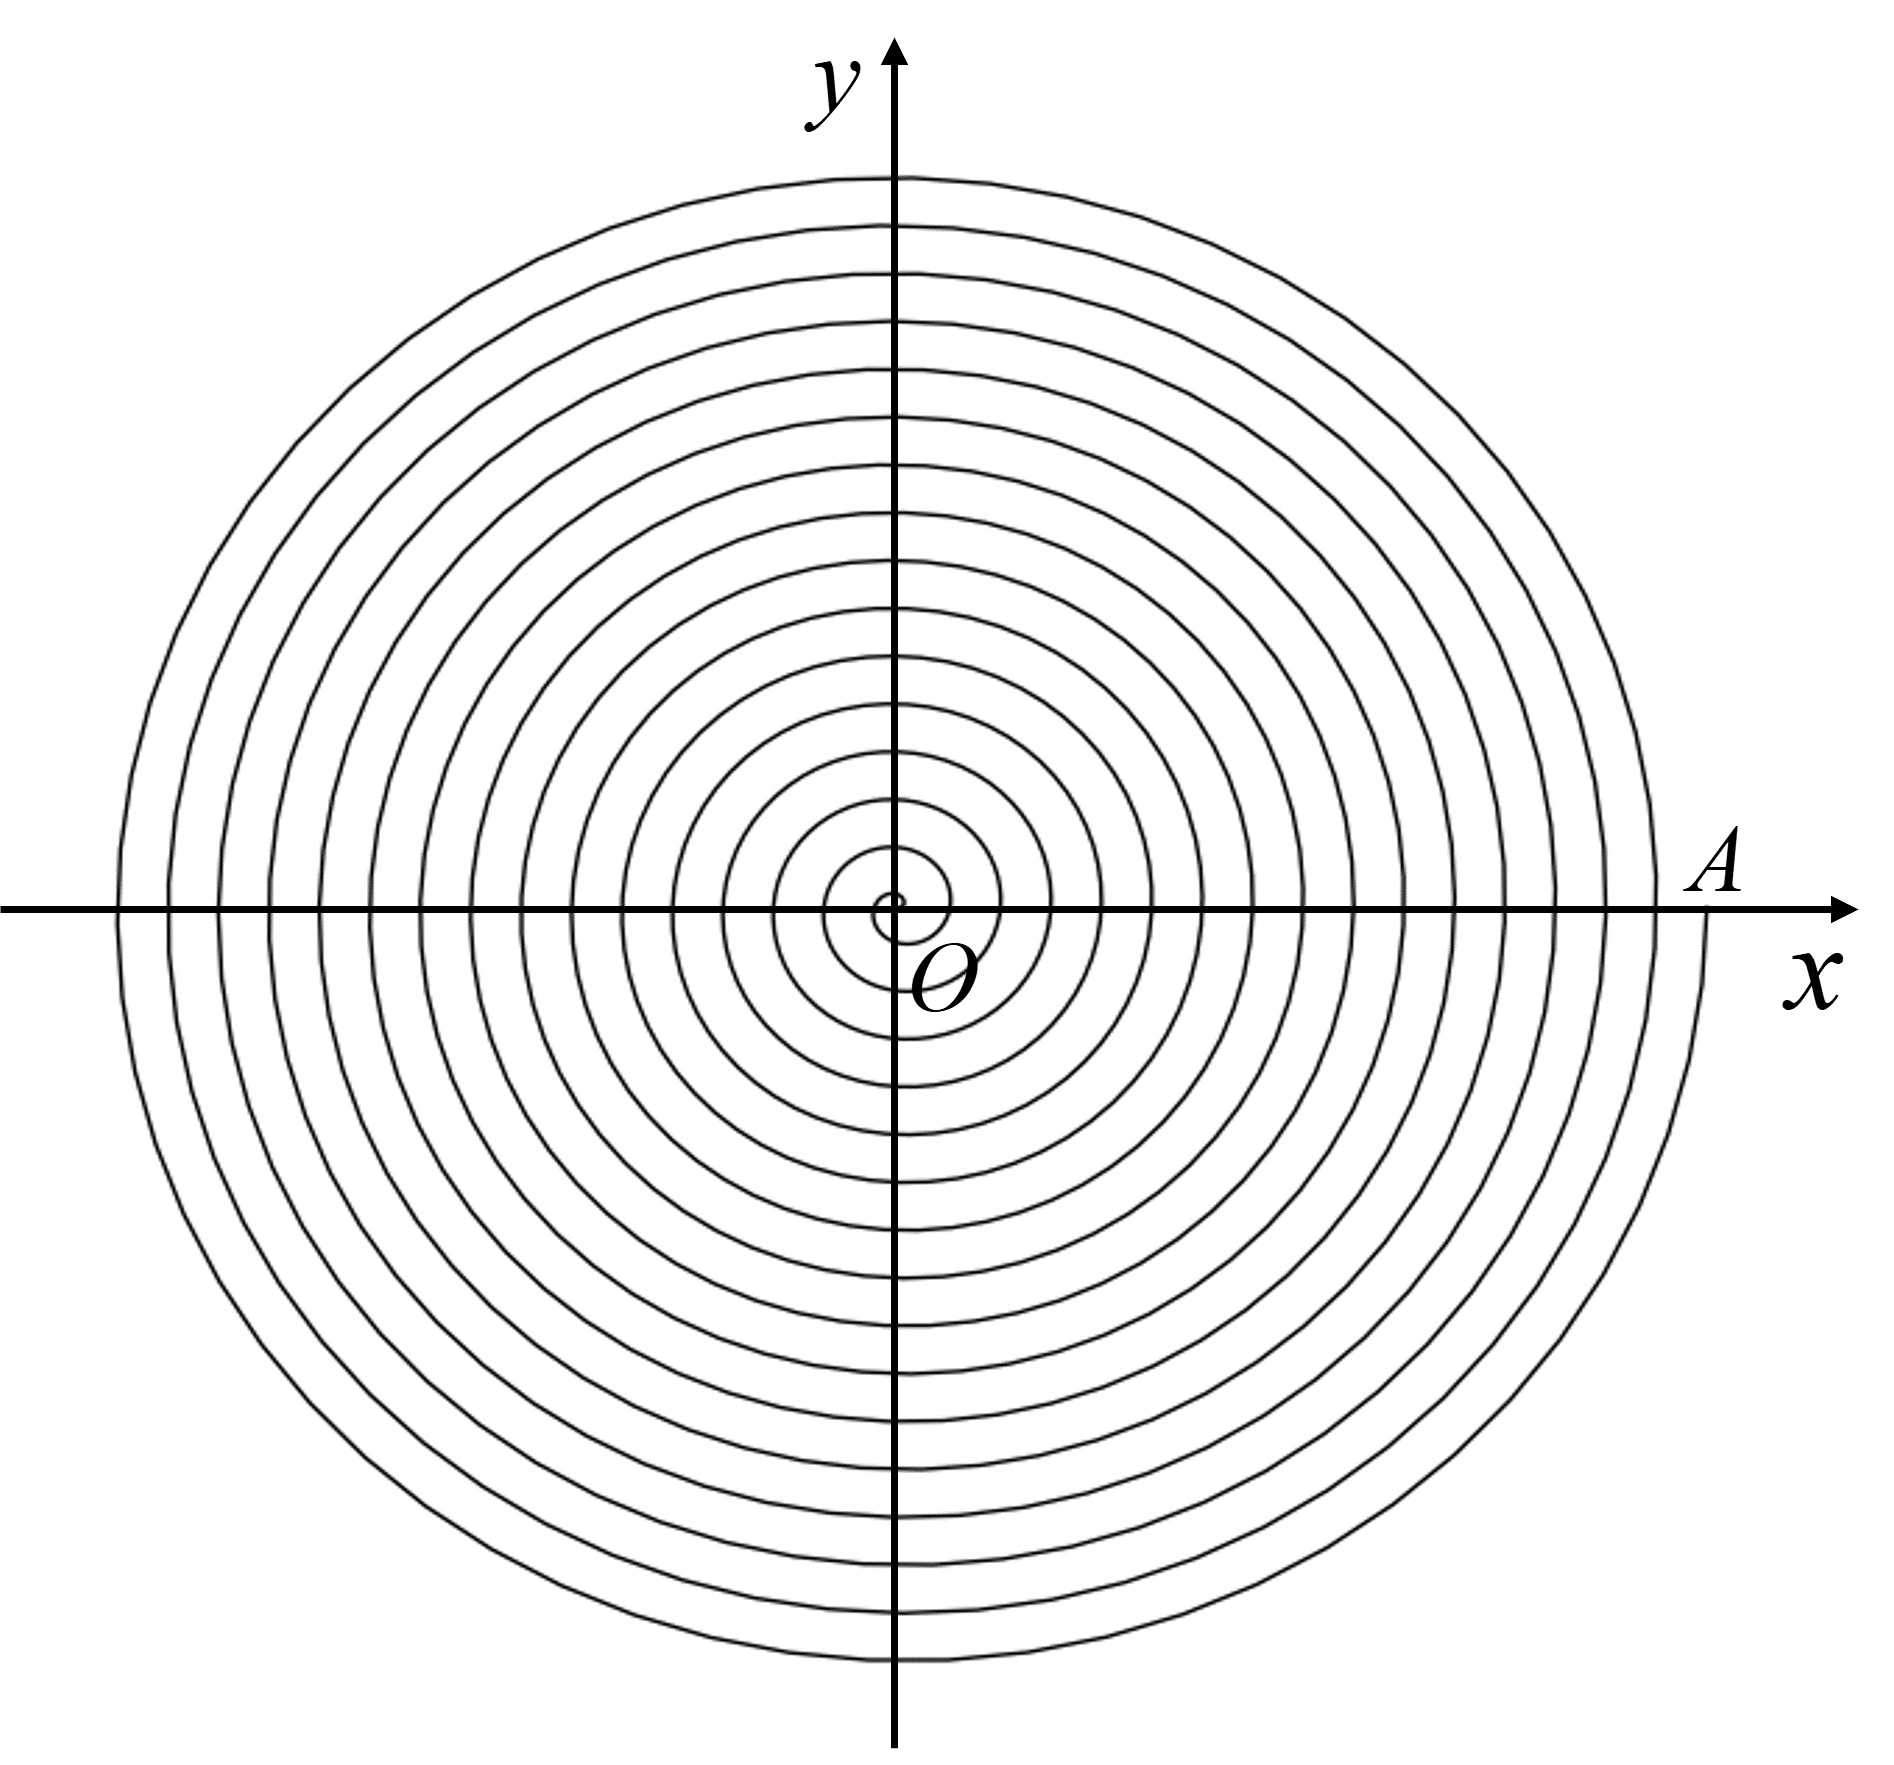
\includegraphics[width=.42\textwidth]{坐标系.png}
		\caption{盘入螺线坐标系示意图}
		\label{坐标系} %在标题之下
	\end{figure}
	问题一中初始时,龙头位于螺线第16圈$A$点处,龙头前把手以恒定初速度$v_h$顺时针进入等距螺线并做匀线速度运动,舞龙队行进时各把手中心均位于螺线上。
	
	\textbf{2.龙头前把手运动状态分析}
	
	由等距螺线的性质\cite{1}可知等距螺旋线上任一点的极径为:
	\begin{equation}
		r=b\theta=\dfrac{d}{2\pi}\theta
	\end{equation}
	其中$d$为等距螺线的螺距,$\theta$为从原点位置绕到目标位置沿等距螺线所绕过的总角度。
	
	得到任一点的极径后,在$d\theta_h$这一微分范围内可以将该运动看作圆弧,故可以计算龙头在任一位置的角速度表达式:
	\begin{equation}
		\omega_h=\dfrac{v_h}{r}
	\end{equation}
	其中,$v_h$为龙头在任一位置的线速度。
	
	角速度的微分形式为:
	\begin{equation}
		\omega_h=\dfrac{d\theta_h}{dt}
	\end{equation}
	其中,$\theta_h$表示从螺线中心开始,沿螺线旋转到龙头前把手位置转过的角度。
	
	联立式(1)(2)(3)可得:
	\begin{equation}
		\begin{cases}
			-\theta_hd\theta_h=\dfrac{2\pi v_h}{d}dt\\
			\theta_h(0)=16\cdot 2\pi
		\end{cases}
	\end{equation}
	
	由初值可解得龙头前把手转过角度随时间变化的表达式为:
	\begin{equation}
		\theta_h=\sqrt{1024\pi ^2-\dfrac{4\pi v_ht}{d}}
	\end{equation}
	计算时,排除$\theta_h$为负的增根。
	\subsubsection{模型建立}
	\textbf{1.对龙头前把手运动状态的建模}
	
	龙头前把手在任意时刻的极径$r_h$和角度$\theta_h$的关系可以表示为:
	\begin{equation}
		r_h=\dfrac{d}{2\pi}\theta_h
	\end{equation}
	
	由此可得龙头前把手在任意时刻的位置为:
	\begin{equation}
		\begin{cases}
			x_h=r_hcos\theta_h\\
			y_h=r_hsin\theta_h
		\end{cases}
	\end{equation}
	
	龙头前把手的运动速度恒定为$v_h$。
	
	\textbf{2.对龙头后第一节龙身运动状态的建模}
	
	当舞龙队进入等距螺线时示意图如图\ref{盘入}所示:
	\begin{figure}[H]
		\centering
		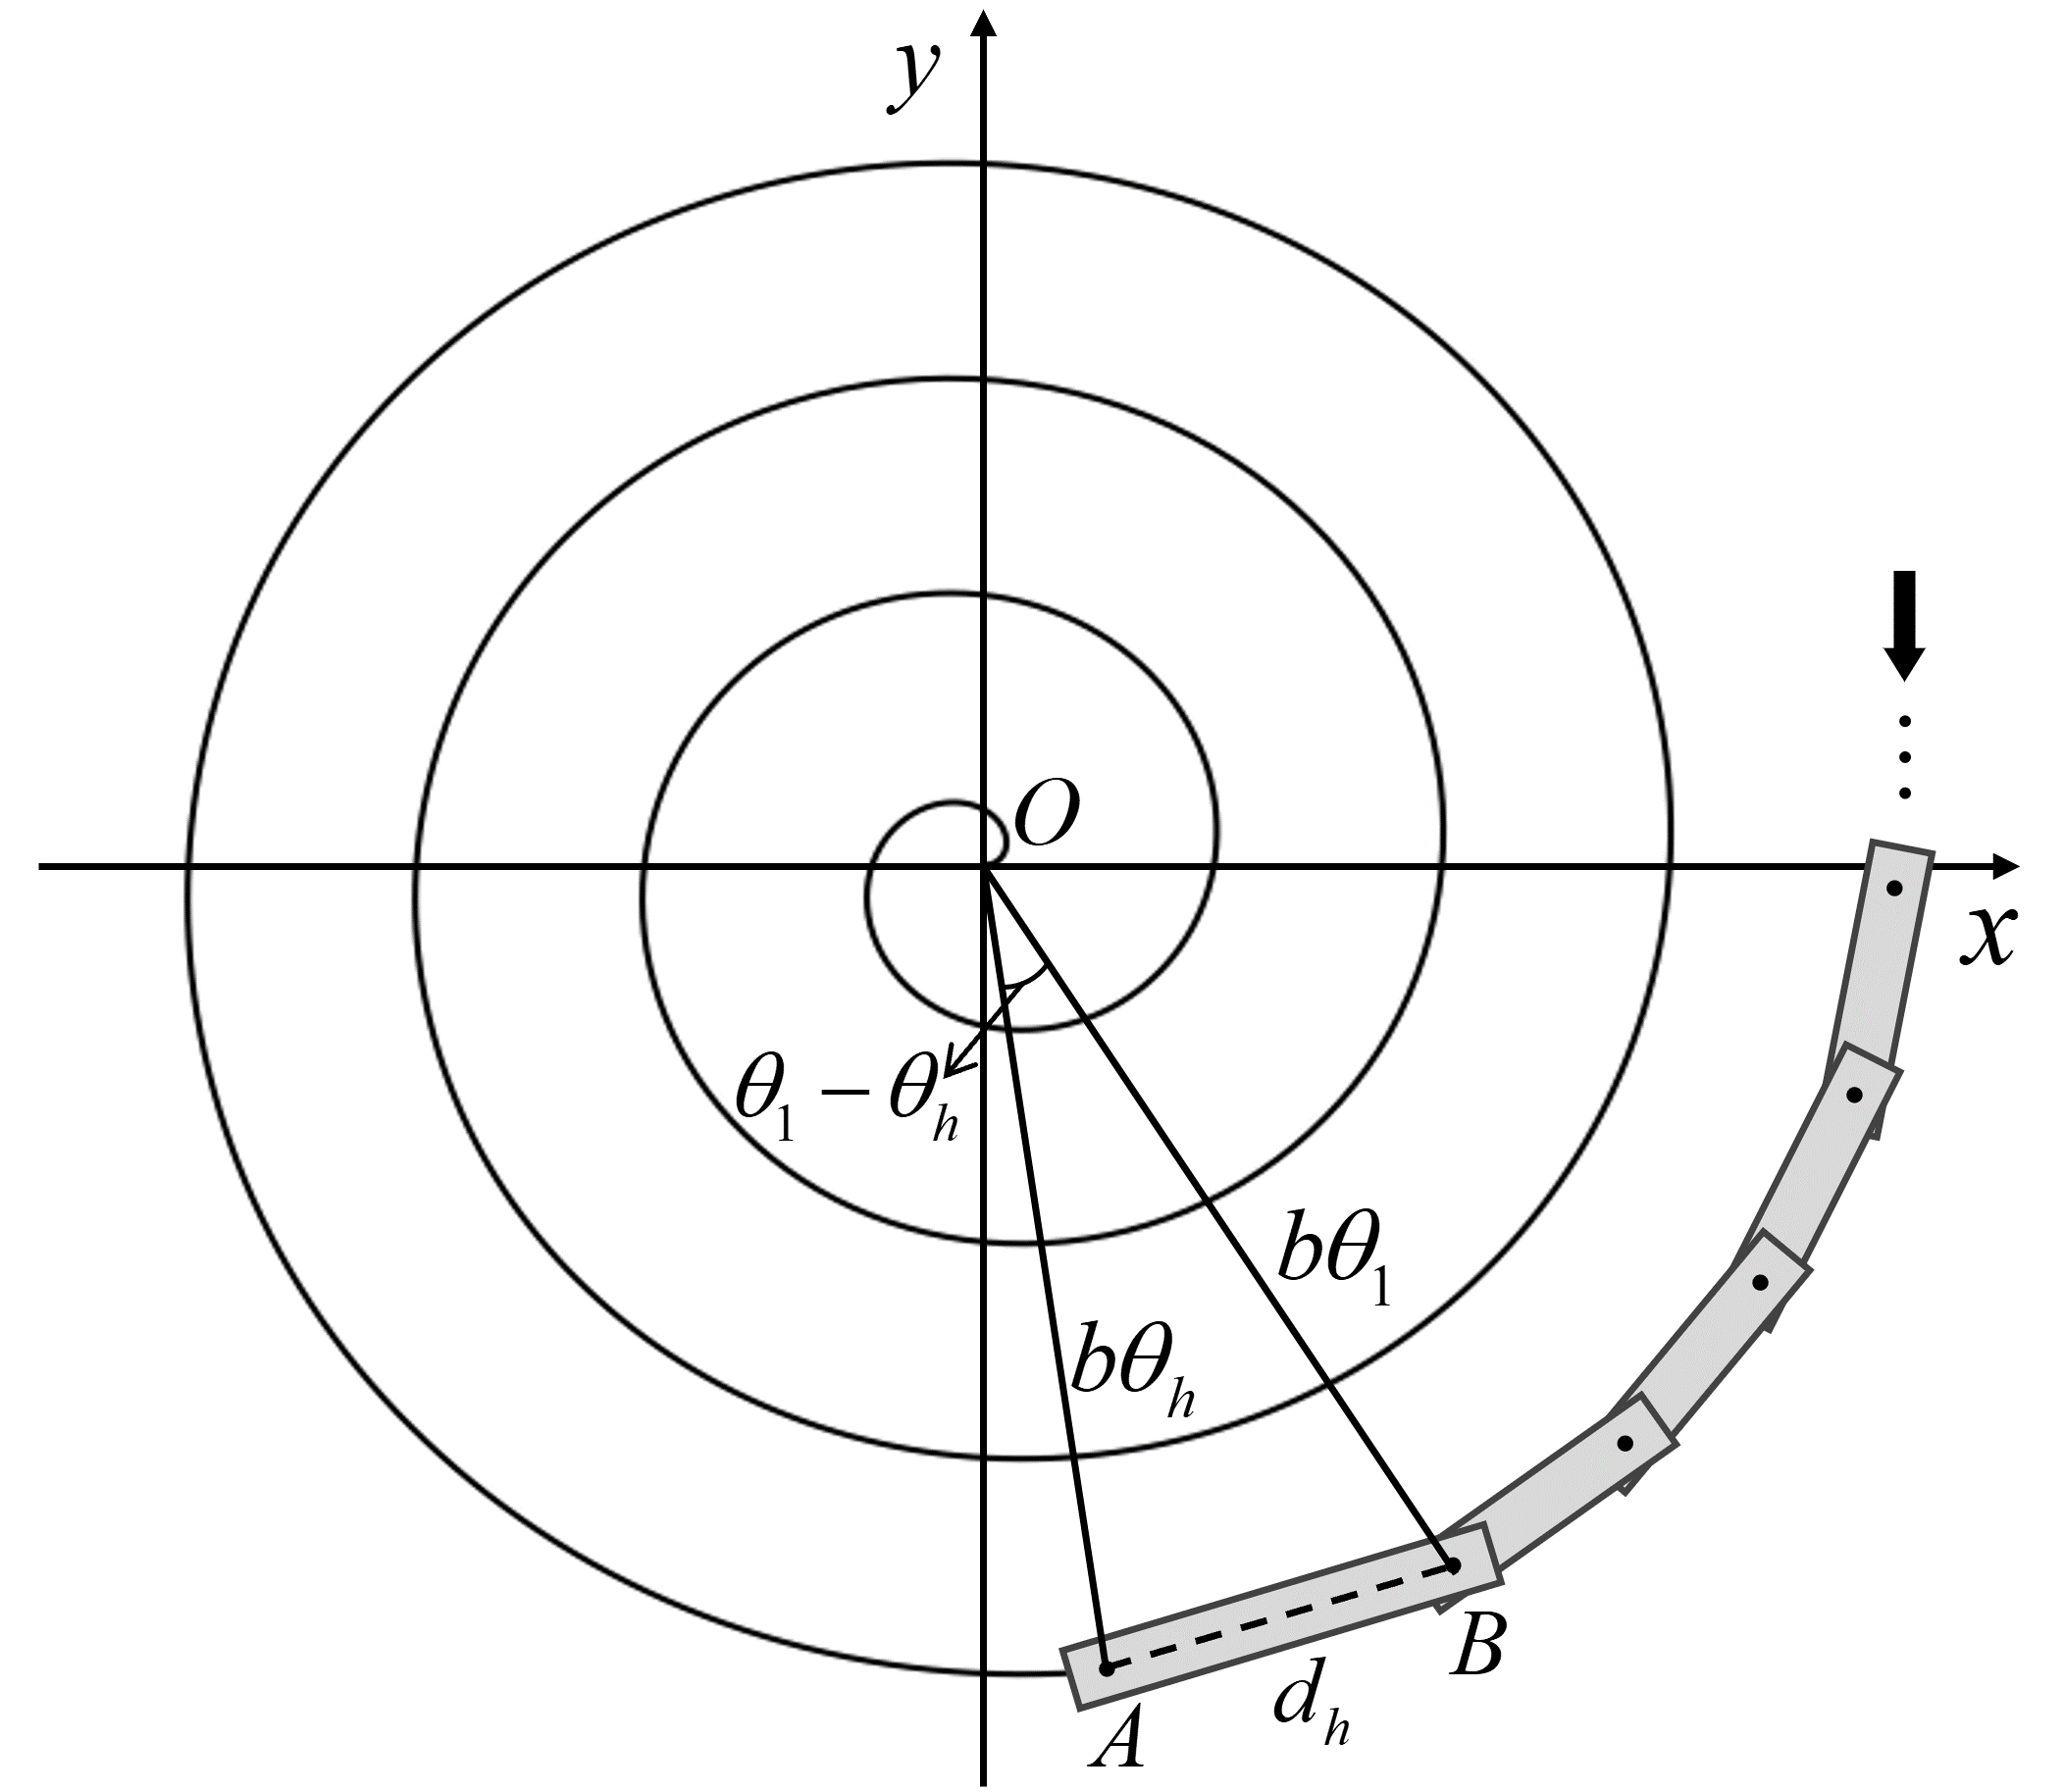
\includegraphics[width=.45\textwidth]{盘入示意图.png}
		\caption{沿等距螺线盘入示意图}
		\label{盘入} %在标题之下
	\end{figure}
	对三角形$OAB$由余弦定理\cite{2}可得:
	\begin{equation}
		cos(\theta_1-\theta_h)=\dfrac{(b\theta_1)^2+(b\theta_h)^2-d^2_h}{2b\theta_1\cdot b\theta_h}
	\end{equation}
	其中,$\theta_1$为龙头后面第一节龙身前把手角度,$d_h$为龙头两个孔心之间的距离。
	
	由于式(8)中只有$\theta_1$一个未知量,本文采用数值分析牛顿迭代法可以求得一元未知方程的解$\theta_1$。
	
	\textbf{3.对龙身运动状态的建模}
	
	对于后续龙身位置的计算,同样可以在龙身两孔心与坐标系原点构成的三角形中利用余弦定理:
	\begin{equation}
		cos(\theta_{i+1}-\theta_i)=\dfrac{(b\theta_{i+1})^2+(b\theta_i)^2-d^2_b}{2b\theta_{i+1}\cdot b\theta_i}
	\end{equation}
	其中$\theta_{i+1}$为龙头后第$i+1$节龙身的前把手($\theta_{223}$表示龙尾的后把手),$\theta_i$为龙头后第$i$节龙身的前把手,$d_b$为龙身两个孔心之间的距离。
	
	式(9)中$\theta_i$可由前一节把手求出,因此只有$\theta_{i+1}$一个未知量,同样由牛顿迭代法可以递推求得一元未知方程的解$\theta_{i+1}$。
	
	对于各把手的速度,可由龙头前把手的速度递推求得,速度模型示意图如图\ref{速度}所示:
	\begin{figure}[H]
		\centering
		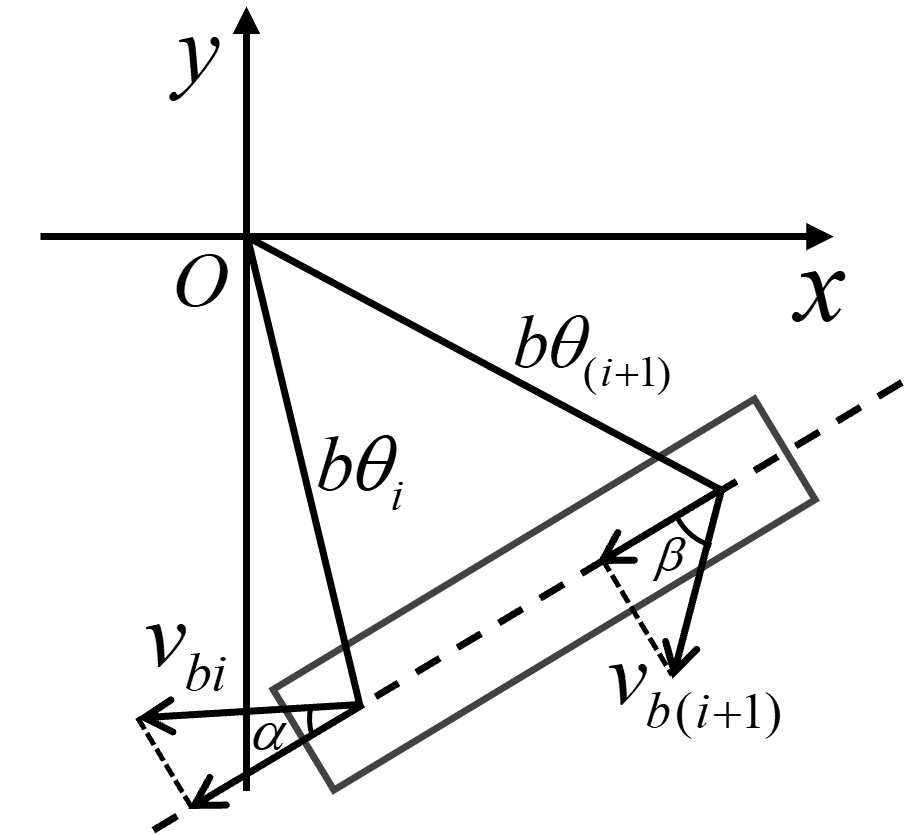
\includegraphics[width=.3\textwidth]{速度沿板.png}
		\caption{速度模型示意图}
		\label{速度} %在标题之下
	\end{figure}
	由于各把手时刻位于等距螺线上且沿螺线运动,因此运动速度方向均沿等距螺线在该点的切线方向,速度分量沿板方向相等:
	\begin{equation}
		v_{bi}cos\alpha=v_{b(i+1)}cos\beta
	\end{equation}
	其中,$v_{bi}$表示龙头后第$i$节龙身前把手的速度。
	
	在等距螺线中:
	\begin{equation}
		\begin{cases}
			x=b\theta cos\theta\\
			y=b\theta sin\theta
		\end{cases}
	\end{equation}
	
	对$\theta$分别求导得:
	\begin{equation}
		\begin{cases}
			\vspace{\topsep}
			\dfrac{dx}{d\theta}=-b\theta sin\theta +bcos\theta\\
			\dfrac{dy}{d\theta}=b\theta cos\theta +bsin\theta
		\end{cases}
	\end{equation}
	
	由式(12)可得螺线在任意一处的切线斜率为:
	\begin{equation}
		m=\dfrac{dx}{dy}=\dfrac{b\theta cos\theta+bsin\theta}{-b\theta sin\theta+bcos\theta}
	\end{equation}
	将板中把手的坐标代入式(13)可得$m_i$,表示该时刻龙头后第$i$节龙身前把手速度所在直线的斜率。由两个把手的坐标可以确定连线的斜率:
	\begin{equation}
		k=\dfrac{dx}{dy}=\dfrac{y_{b(i+1)}-y_{bi}}{x_{b(i+1)}-x_{bi}}
	\end{equation}

	故在式(10)中,角$\alpha$和角$\beta$可表示为:
	\begin{equation}
		\begin{cases}
			\alpha=tan^{-1}k-tan^{-1}m_i\\
			\beta=tan^{-1}m_{i+1}-tan^{-1}k
		\end{cases}
	\end{equation}
	
	综上,龙身运动状态模型如式(16):
	\begin{equation}
		\begin{cases}
			\setlength\abovedisplayskip{5pt}
			\setlength\belowdisplayskip{5pt}
			x_{bi}=r_icos\theta_i\\
			y_{bi}=r_isin\theta_i\\
			\dfrac{v_{b(i+1)}}{v_{bi}}=\dfrac{cos\alpha_{(i+1)}}{cos\beta_i}
		\end{cases}
	\end{equation}
	代入龙头前把手初速度$v_h$可递推求得舞龙队各部分速度。
	\subsubsection{模型求解}
	在问题一中已知参数见表\ref{参数}:
	\begin{table}[H]
		\centering
		\setlength\extrarowheight{-2pt}
		\setlength{\tabcolsep}{28pt}
		\caption{问题一已知参数} 
		\label{参数} 
		\begin{tabular}{ccccc}
			\specialrule{1.5pt}{0pt}{0pt}
			参数&$d$& $v_h$   & $d_h$   & $d_b$   \\
			\specialrule{1pt}{0pt}{0pt}
			数值 &0.55m& 1m/s & 2.86m & 1.65m \\
			\specialrule{1.5pt}{0pt}{0pt}
		\end{tabular}
	\end{table}
	将龙头的初始运动状态代入建立的模型,即可求得所有把手运动状态。通过递推求出从初始时刻到 300 s 为止,每秒整个舞龙队的位置和速度,下述表\ref{问题一位置}和表\ref{问题一速度}分别为0 s、60 s、120 s、180 s、240 s、300 s 时,龙头前把手、龙头后面第 1、51、101、151、201 节龙身前把手和龙尾后把手的位置和速度,具体求解结果见文件 result1.xlsx。
	\begin{table}[H]
		\centering
		\setlength{\tabcolsep}{8pt}
		\caption{问题一舞龙队的位置} 
		\label{问题一位置} 
		\setlength\extrarowheight{-3pt}
		\small
		\begin{tabular}{|c|c|c|c|c|c|c|}
			\hline
			& 0s       &    60s      & 120s & 180s & 240s & 300s \\ \hline
			龙头x(m)     & 8.800000 &   5.796934  & -4.090654 &-2.953259&2.578971& 4.431365\\ \hline
			龙头y(m)      &   0.000000     &  -5.773329  & -6.300643&6.099638 &-5.363954& 2.298233\\ \hline
			第1节龙身x(m)  & 8.363824 &  7.455390   &-1.452253 & -5.229685 &4.810833& 2.480900     \\ \hline
			第1节龙身y(m)  & 2.826544 & -3.443281  & -7.404474& 4.368312 &-3.575548 & 4.389951     \\ \hline
			第51节龙身x(m) & -9.518736 & -8.685398 &-5.537887&2.901007 &5.970603&-6.299130 \\ \hline
			第51节龙身y(m) & 1.341112   & 2.543141 & 6.382421 &7.244935& -3.842026 & 0.490490     \\ \hline
			第101节龙身x(m) & 2.914039   & 5.684538 & 5.356285&1.887650 &-4.930766&  -6.224242    \\ \hline
			第101节龙身y(m) &  -9.918295 & -8.003181&-7.561567 &-8.473987 &-6.369293& 3.956744     \\ \hline
			第151节龙身x(m) &  10.861711 & 6.684695 & 2.395398&1.016445& 2.981390& 7.053566     \\ \hline
			第151节龙身y(m) & 1.828852   & 8.132552 & 9.725716&9.423434 &8.393873& 4.371895     \\ \hline
			第201节龙身x(m) &  4.554963  & -6.617181 &-10.626288 &-9.292339&-7.467880 & -7.472671     \\ \hline
			第201节龙身y(m) & 10.725178  & 9.027361 & 1.366600 &-4.236322&-6.167517& -5.243064     \\ \hline
			龙尾(后)x(m) & -5.305286   & 7.362212 &10.974813 &7.391885& 3.257083& 1.809208     \\ \hline
			龙尾(后)y(m) & -10.676664  & -8.799924&0.836694&7.484356 &9.463677& 9.296260   \\ \hline
		\end{tabular}
	\end{table}
	\vspace{-0.5cm} 
	\begin{table}[H]
		\centering
		\setlength{\tabcolsep}{10pt}
		\caption{问题一舞龙队的速度} 
		\label{问题一速度} 
		\setlength\extrarowheight{-3pt}
		\small
		\begin{tabular}{|c|c|c|c|c|c|c|}
			\hline
			& 0s & 60s & 120s & 180s & 240s & 300s \\ \hline
			龙头(m/s)     &  1.000000  & 1.000000 & 1.000000 & 1.000000 & 1.000000 & 1.000000 \\ \hline
			第1节龙身(m/s)  &  0.999971  & 0.999961 & 0.999945& 0.999917 & 0.999859 & 0.999709     \\ \hline
			第51节龙身(m/s) &  0.999744 &0.999663 & 0.999537 & 0.999331 &0.998939 & 0.998066     \\ \hline
			第101节龙身(m/s)   & 0.999578  &0.999450&0.999266&0.998972&0.998433 & 0.997302     \\ \hline
			第151节龙身(m/s)   &  0.999452  &0.999298& 0.999078 & 0.998730 &0.998113&  0.996861    \\ \hline
			第201节龙身(m/s)   & 0.999352 &0.999183&0.998929& 0.998556& 0.997892& 0.996573     \\ \hline
			龙尾(后)(m/s)   & 0.999308 &0.999139& 0.998883 & 0.998490 &0.997816&  0.996478  \\ \hline
		\end{tabular}
	\end{table}
	\subsubsection{结果分析}	
	在问题一中,舞龙队中可能出现同一个板子的两个孔处于套圈位置如图\ref{特殊}所示:
	\begin{figure}[H]
		\centering
		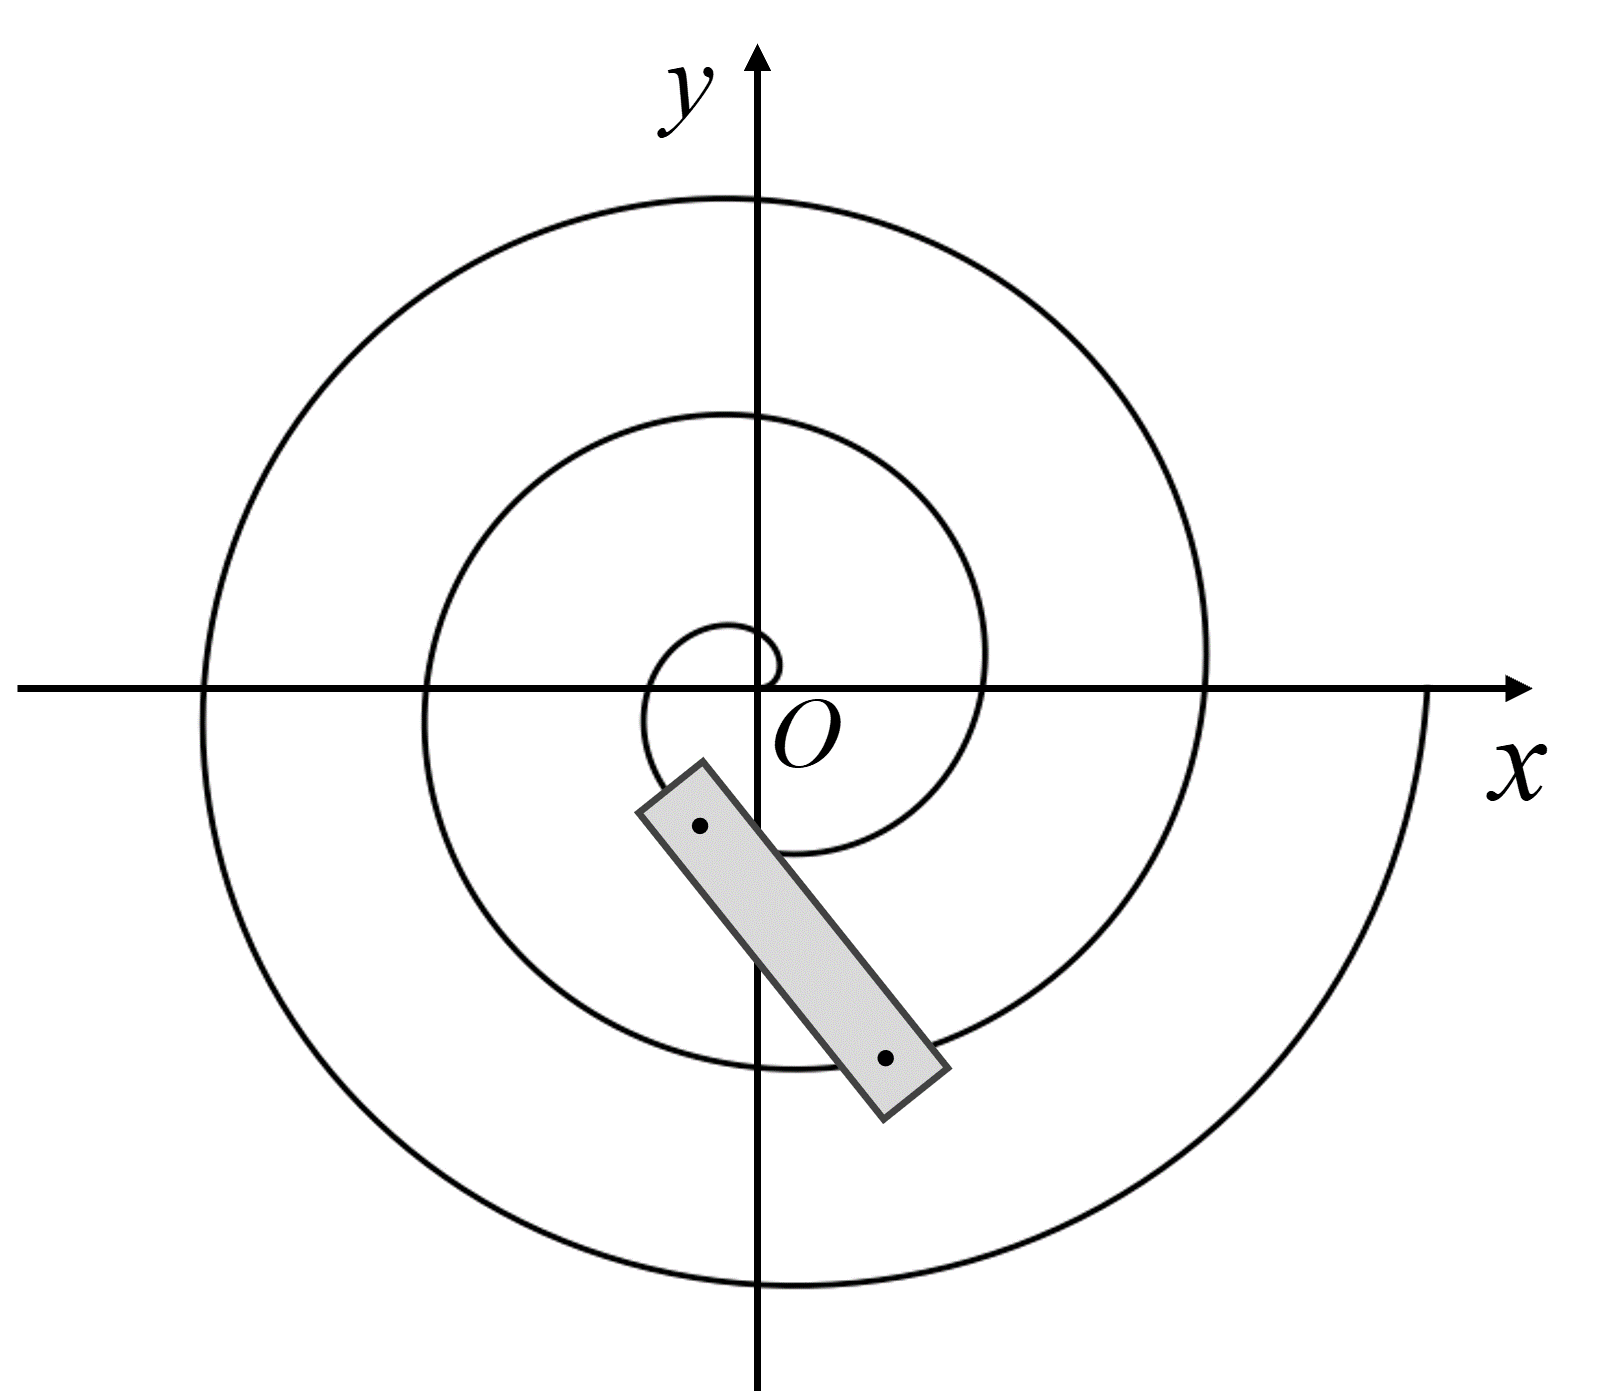
\includegraphics[width=.35\textwidth]{特殊情况.png}
		\caption{两孔处于套圈状态示意图}
		\label{特殊} %在标题之下
	\end{figure}
	该情况导致该方程可能有多个解,本文假设在问题一中不会出现这种错位,而我们需要的是所有比$\theta_h$大的解中最小的那个解,因此在牛顿迭代法中选择一个合理的初值是十分有必要的,本文在实际计算中选择了$\theta_1+\dfrac{\pi}{2}$作为牛顿迭代法的初值,最后对求解得到的龙头位置结果进行检查,通过观察发现龙头前把手和龙头后第一节龙身前把手角度之差和相邻两节龙身前把手之差均远远小于$2\pi$,因此假设成立。

	\subsection{问题二的模型建立与求解}
	\subsubsection{模型准备}
	\textbf{1.终止时刻的确定}
	
	当舞龙队沿问题一中的等距螺线盘入时,可能会发生碰撞如图\ref{碰撞}所示:
	\begin{figure}[H]
		\centering
		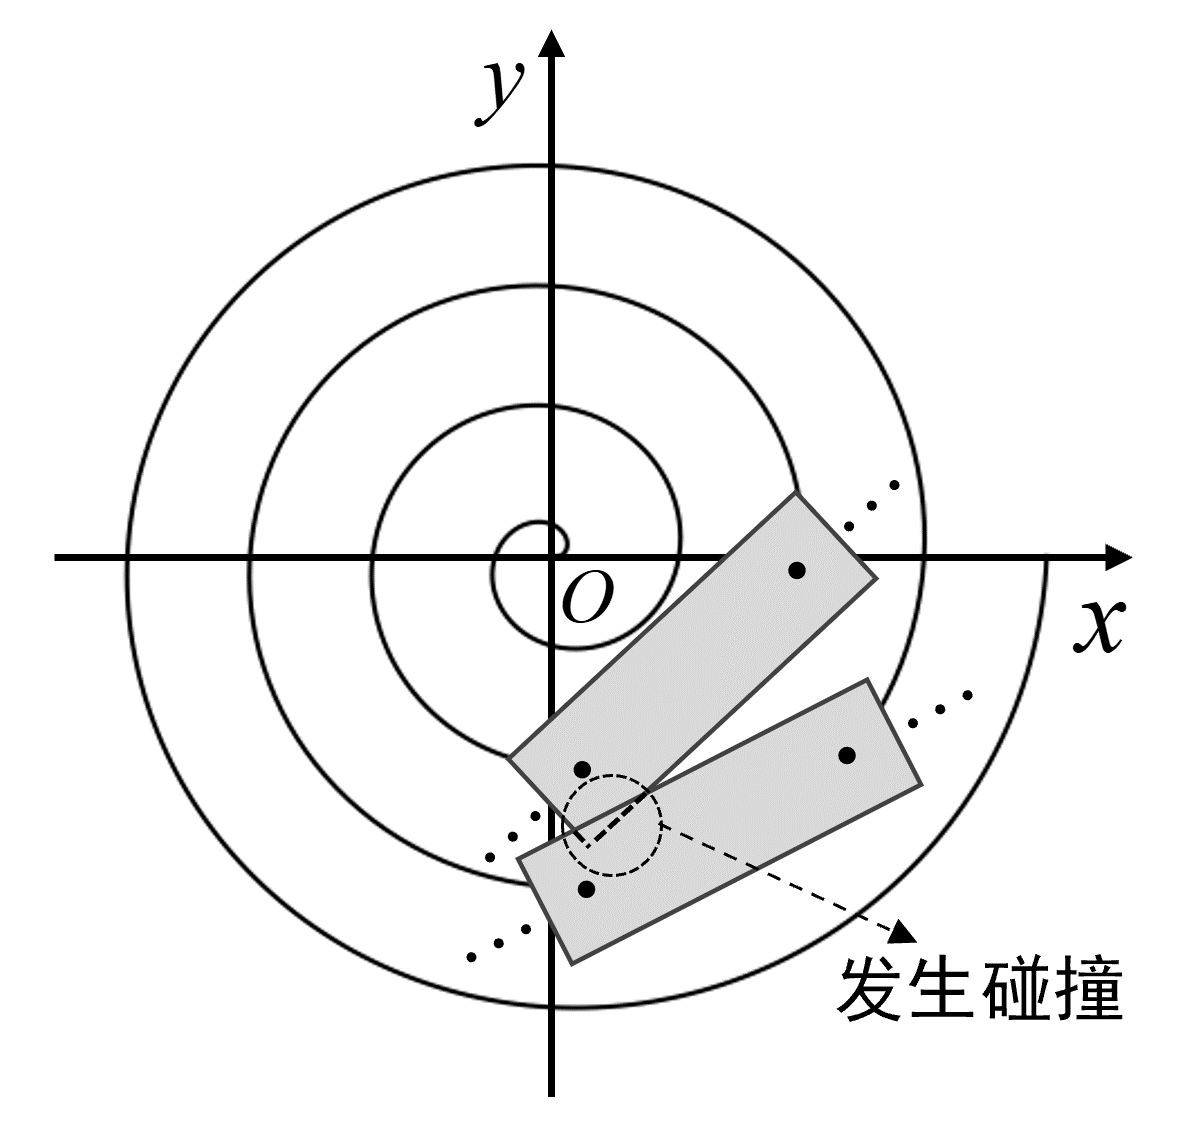
\includegraphics[width=.38\textwidth]{碰撞.png}
		\caption{板凳间发生碰撞示意图}
		\label{碰撞} %在标题之下
	\end{figure}
	当舞龙队中有碰撞恰好发生时,我们确定此时刻为舞龙队盘入的终止时刻,记录舞龙队在终止时刻的位置和速度信息。
	
	\textbf{2.求解龙头矩形边界点}
	
	龙头的两个孔心的坐标位置可由问题一模型确定,假设龙头在某一时刻所在位置如图\ref{辅助线}所示:
	\begin{figure}[H]
		\centering
		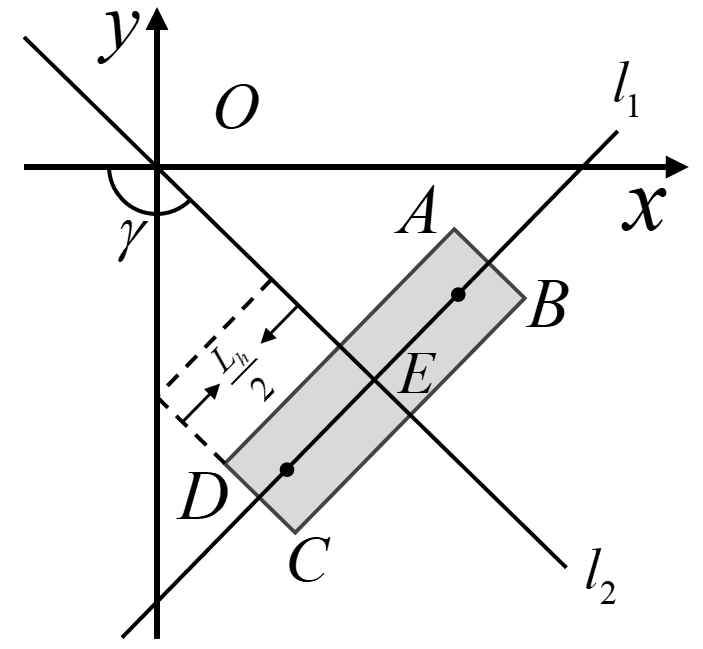
\includegraphics[width=.3\textwidth]{辅助线.png}
		\caption{龙头位置描述示意图}
		\label{辅助线} %在标题之下
	\end{figure}
	图中直线$l_1$可由两孔心坐标确定,设两孔心坐标分别为$(x_{h1},y_{h1})$、$(x_{h2},y_{h2})$,两点的中点坐标为$E(x_0,y_0)$,则直线$l_1$的方程可表示为:
	\begin{equation}
		y=\dfrac{y_{h2}-y_{h1}}{x_{h2}-x_{h1}}(x-x_{h1})+y_{h1}
	\end{equation}
	中点坐标可表示为:
	\begin{equation}
		\begin{cases}
			\vspace{\topsep}
			x_0=\dfrac{x_{h1}+x_{h2}}{2}\\
			y_0=\dfrac{y_{h1}+y_{h2}}{2}
		\end{cases}
	\end{equation}
	
	过中点作直线$l_1$的垂线$l_2$,斜率存在关系如下:
	\begin{equation}
		k_1\cdot k_2=-1
	\end{equation}
	
	故可确定直线$l_2$的方程:
	\begin{equation}
		y=-\dfrac{x_{h2}-x_{h1}}{y_{h2}-y_{h1}}(x-x_0)+y_0
	\end{equation}
	
	通过平移直线$l_1$、$l_2$,可以得到龙头矩阵边界直线的方程如下:
	\begin{equation}
		\begin{cases}
			\vspace{\topsep}
			AB:y=k_1(x-x_{h1})+y_{h1}+\dfrac{W_h}{2}\sqrt{1+k_1^2}\\
			\vspace{\topsep}
			CD:y=k_1(x-x_{h1})+y_{h1}-\dfrac{W_h}{2}\sqrt{1+k_1^2}\\
			\vspace{\topsep}
			BC:y=k_2(x-x_0)+y_0+\dfrac{L_h}{2}\sqrt{1+(tan(\pi-\gamma))^2}\\
			DA:y=k_2(x-x_0)+y_0-\dfrac{L_h}{2}\sqrt{1+(tan(\pi-\gamma))^2}\\
		\end{cases}
	\end{equation}
	其中,
	\begin{equation}
		tan(\pi-\gamma)=-tan\gamma=-k_2
	\end{equation}
	
	通过联立四条直线方程(21)和式(22)可以求得龙头板凳四个顶点在该时刻的坐标分别为$(x_A,y_A)$、$(x_B,y_B)$、$(x_C,y_C)$、$(x_D,y_D)$。
	
	\textbf{3.求解龙身矩形边界点}
	
	龙身矩形边界点求解方法与龙头相同,只需将板长和板宽参数需要更换为龙身板凳参数$L_b$、$W_b$,其余求解过程与龙头边界点求解相同在此处不再赘述。
	\subsubsection{模型建立}
	\textbf{1.碰撞条件判断}
	
	由图\ref{碰撞}所示碰撞时刻可知,发生碰撞时会出现一个板凳的顶点落入另一块板凳区域中,通过遍历判断每一个板凳的四个顶点是否落在除相邻板凳外其他板凳区域中来判断该板凳是否发生碰撞。
	
	\textbf{2.顶点发生碰撞的条件}
	
	首先考虑顶点是否在板宽的范围内,先求解一顶点到任一非相邻板的把手连线所在直线的距离$D$,如果该距离$D$满足以下关系:
	\begin{equation}
		D\le \dfrac{W_b}{2}
	\end{equation}
	说明顶点落在板凳之外,不发生碰撞;否则,考虑顶点是否在长方形长度的范围内,此时求解顶点在相邻把手之间的投影,如果投影位置到两把手之间距离之和$l$大于板凳长,说明顶点落在板凳之外,不发生碰撞,否则说明顶点落在板凳之内,发生碰撞。
	\begin{figure}[H]
		\centering
		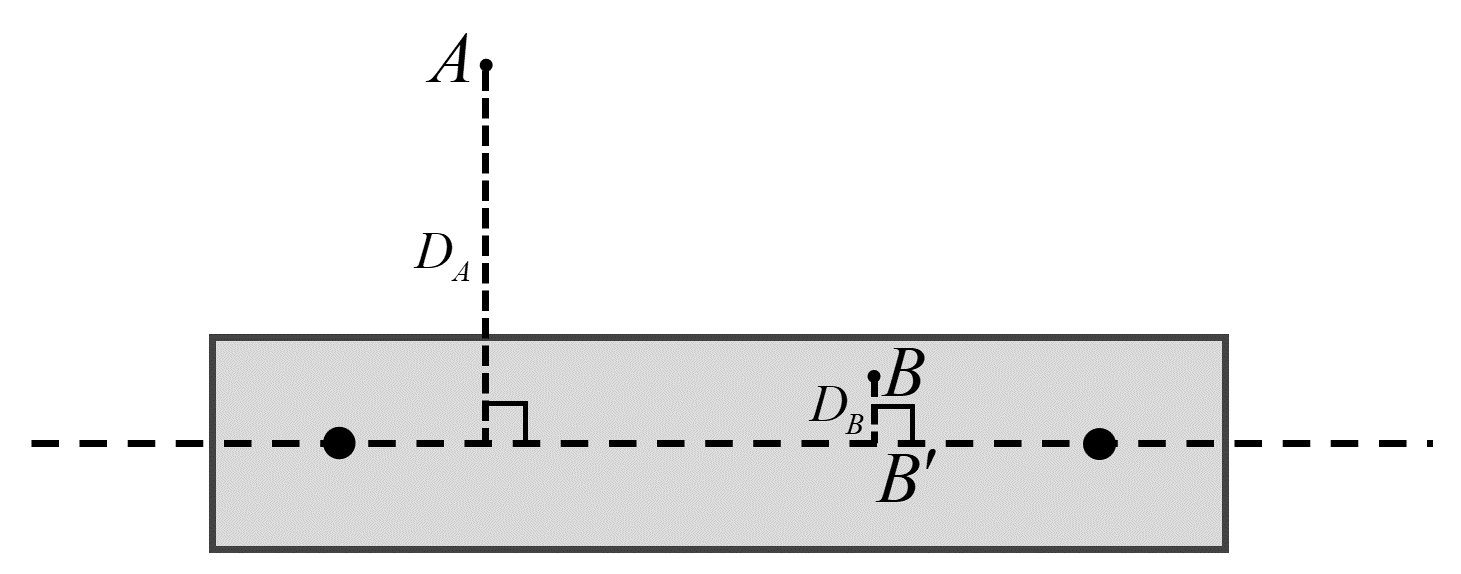
\includegraphics[width=.45\textwidth]{垂线.png}
		\caption{判断顶点发生碰撞示意图}
		\label{垂线} %在标题之下
	\end{figure}
	其中,$D$和$l$可由点到直线距离和两点间距离求解。
	\subsubsection{模型求解}
	通过以时间步长为1s遍历判断计算所有板凳的顶点是否落入非相邻板凳区域找到了舞龙队在第413s恰好发生碰撞,此时为龙头和龙头后第8节龙身发生了碰撞,记录此时舞龙队的位置和速度,具体求解结果见文件 result2.xlsx。下述表\ref{问题二位置和速度}为此时龙头前把手、龙头后面第 1、51、101、151、201 节龙身前把手和龙尾后把手的位置和速度。
	\begin{table}[H]
		\centering
		\setlength{\tabcolsep}{15pt}
		\caption{问题二舞龙队的位置和速度} 
		\label{问题二位置和速度} 
		\setlength\extrarowheight{-1pt}
		%\small
		\begin{tabular}{|c|c|c|c|}
			\hline
			& 横坐标x(m) & 纵坐标y(m) & 速度(m/s) \\ \hline
			龙头x    & 1.647511& 1.556154 &1.000000 \\ \hline
			第1节龙身  &-1.164436&2.078219&0.991145\\ \hline
			第51节龙身 &1.803760&4.119592& 0.976112 \\ \hline
			第101节龙身 &-1.099658&-5.792623&0.973782  \\ \hline
			第151节龙身  &0.401238 & -7.006028&0.972839 \\ \hline
			第201节龙身  & -7.954575 &-0.664687 &0.972327\\ \hline
			龙尾(后)  & 1.518361&8.232690&0.972167 \\ \hline
		\end{tabular}
	\end{table}
	\subsubsection{结果分析}
	通过计算得到了舞龙队的终止时刻,此时舞龙队的位置如图\ref{发生碰撞}所示:
	\begin{figure}[H]
		\centering
		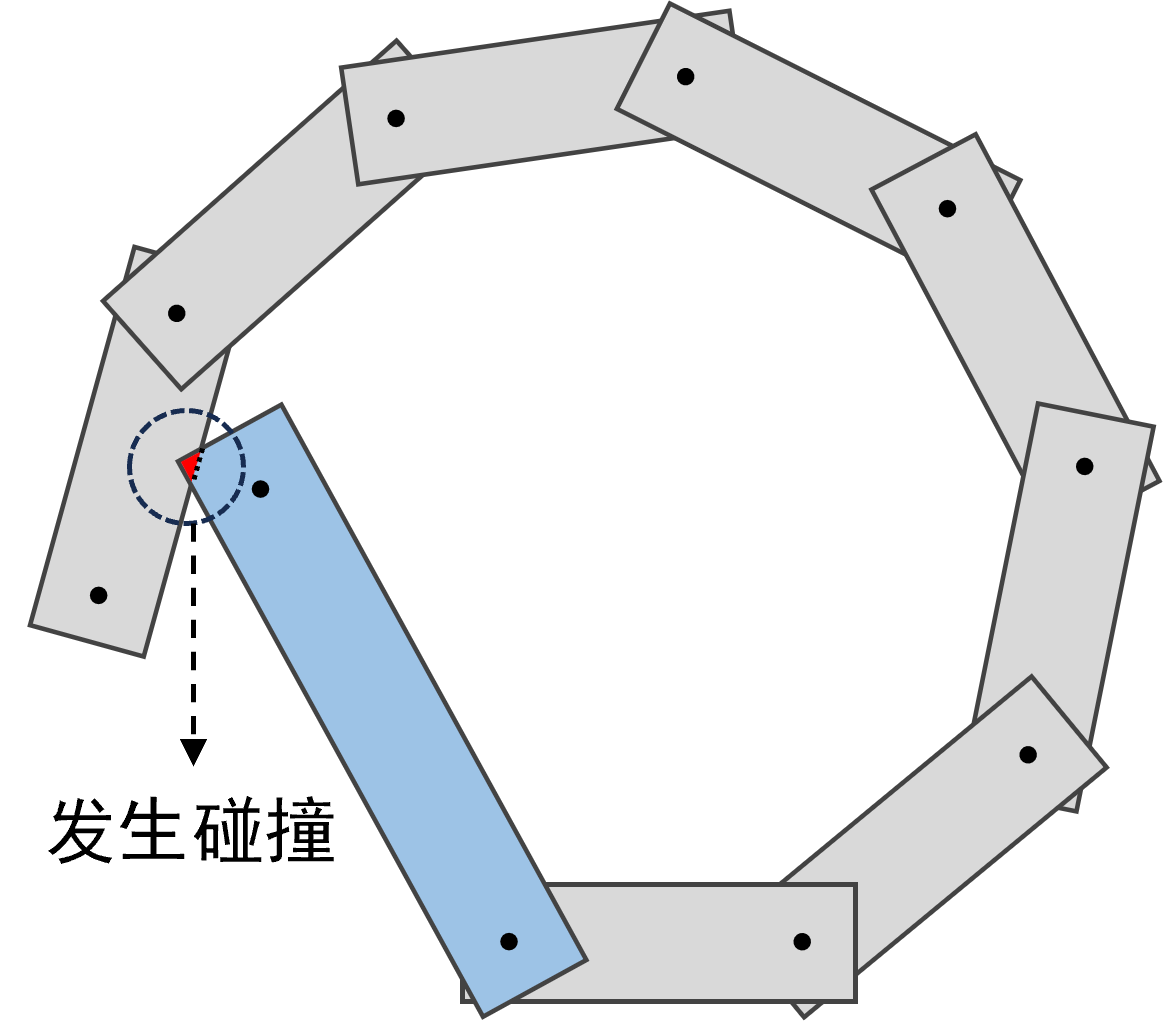
\includegraphics[width=.35\textwidth]{发生碰撞.png}
		\caption{龙头与第8节龙身碰撞示意图}
		\label{发生碰撞} %在标题之下
	\end{figure}
	龙头与龙身发生碰撞时刻即为舞龙队盘入的终止时刻,观察发现,龙头的长度大于龙身,其在螺线中运动时弦长较大,导致碰撞发生。

	\subsection{问题三的模型建立与求解}
	\subsubsection{最小螺距优化模型建立}
	舞龙队调头空间是以螺线中心为圆心,直径为9m的圆,如图\ref{调头空间}所示:
	\begin{figure}[H]
		\centering
		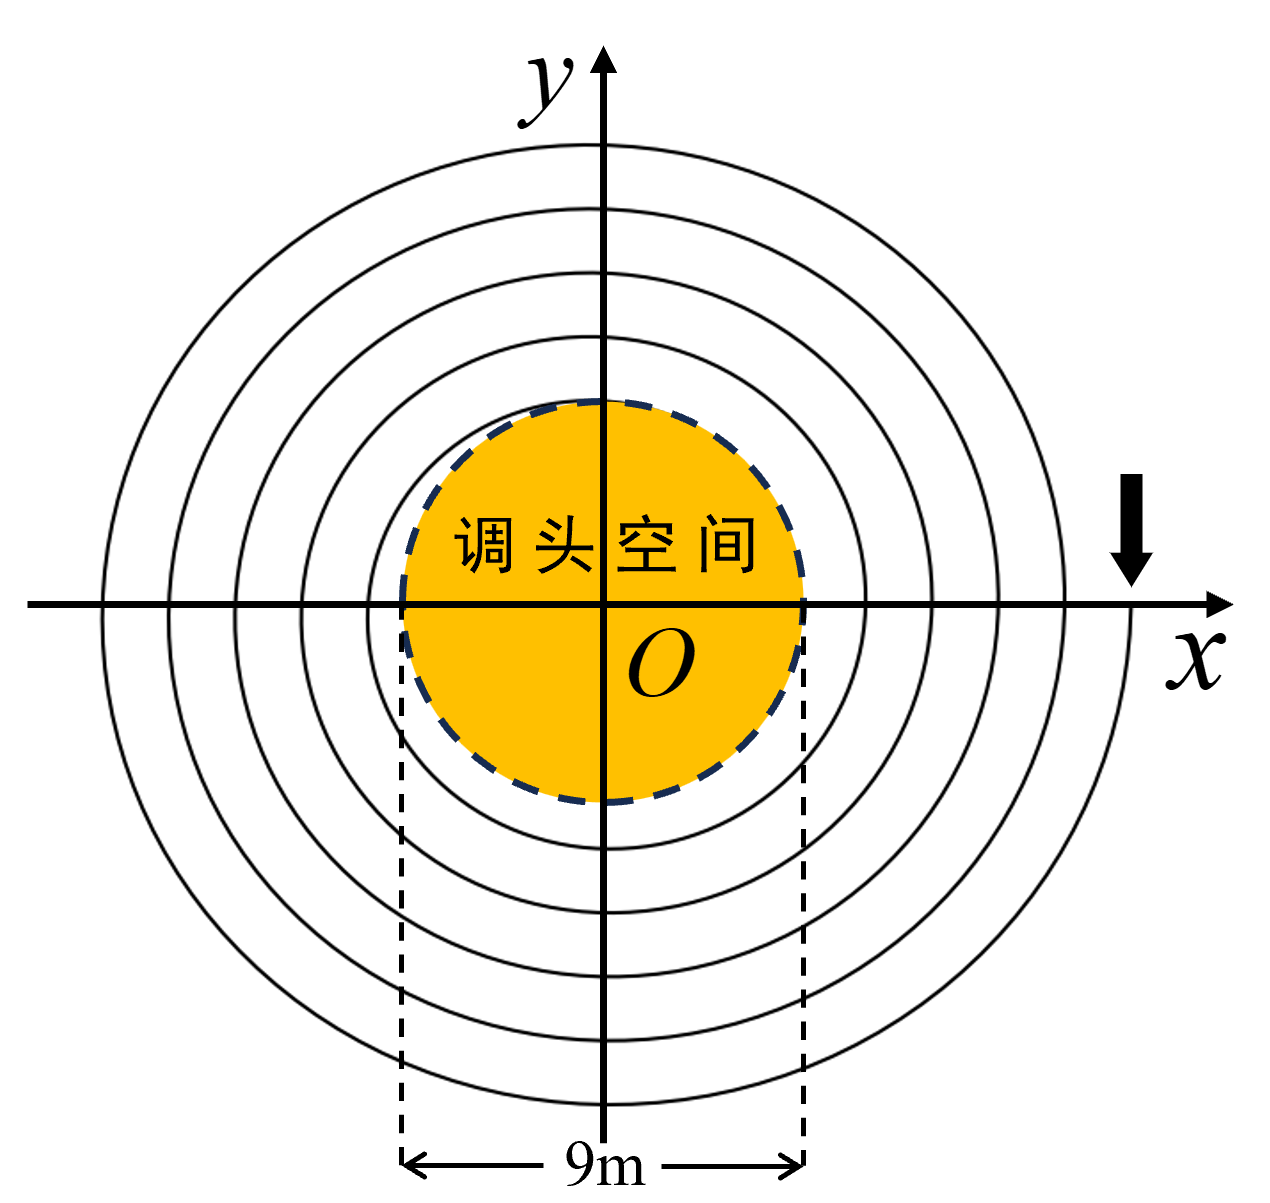
\includegraphics[width=.4\textwidth]{调头空间.png}
		\caption{调头空间示意图}
		\label{调头空间} %在标题之下
	\end{figure}
	发生碰撞时龙头前把手位置坐标为$(x_h,y_h)$,通过比较龙头到原点的距离$d_h$与调头圆半径来判断是否恰好达到边界状态,即螺距$d$最小。
	\begin{equation}
		d_h=\sqrt{x_h^2+y_h^2}
	\end{equation}

	由题目条件得,为保证龙头前把手可按照相应螺线盘入到调头空间的边界,可确定约束条件为:
	\begin{equation}
		\sqrt{x_h^2+y_h^2}\le4.5m
	\end{equation}
	目标函数为:
	\begin{equation}
		\mbox{min} \{d\} 
	\end{equation}
	\subsubsection{最小螺距优化模型求解}
	对于寻找最优解,即最小螺距$d_{min}$,本论文采用变步长遍历和二分算法。由题设容易得到,螺距越小越容易发生碰撞,即碰撞半径随螺距的变化是单调的,因此可以采用二分法求解。由问题一中条件,螺距 $d=0.55$m,发生碰撞时龙头前把手的坐标为 (1.647511,1.556154),到达原点的距离为2.266254,小于调头空间圆半径,故在此以 0.55m 作遍历空间上界。求解具体流程如下:
	
	\textbf{Step1:}设置螺距的遍历范围 $d\in [0, 0.55]$,取步长为 0.01m,进行初次遍历,确定最优解所在区间为$d\in [0.4, 0.5]$。 
	
	\textbf{Step2:}利用二分法进行$n$ 次迭代,当步长之差小于0.001m时跳出循环,找到较小的修正范围。
	
	最后得到结果:
	\begin{equation}
		d_{min}=0.451\mbox{m}
	\end{equation}

	\subsection{问题四的模型建立与求解}
	\subsubsection{模型建立}
	\textbf{1.调头曲线长度模型}
	
	舞龙队在问题三调头空间设定的基础上完成调头,由题目条件可知,调头路径是由两段圆弧相切连接而成的S形曲线,前段圆弧半径是后段的2倍,盘出螺线与盘入螺线关于螺线中心呈中心对称,S形曲线与盘入、盘出螺线均相切。盘入盘出曲线(左)和调头曲线(右)如图\ref{问题四}所示:
	\begin{figure}[H]
		\centering
		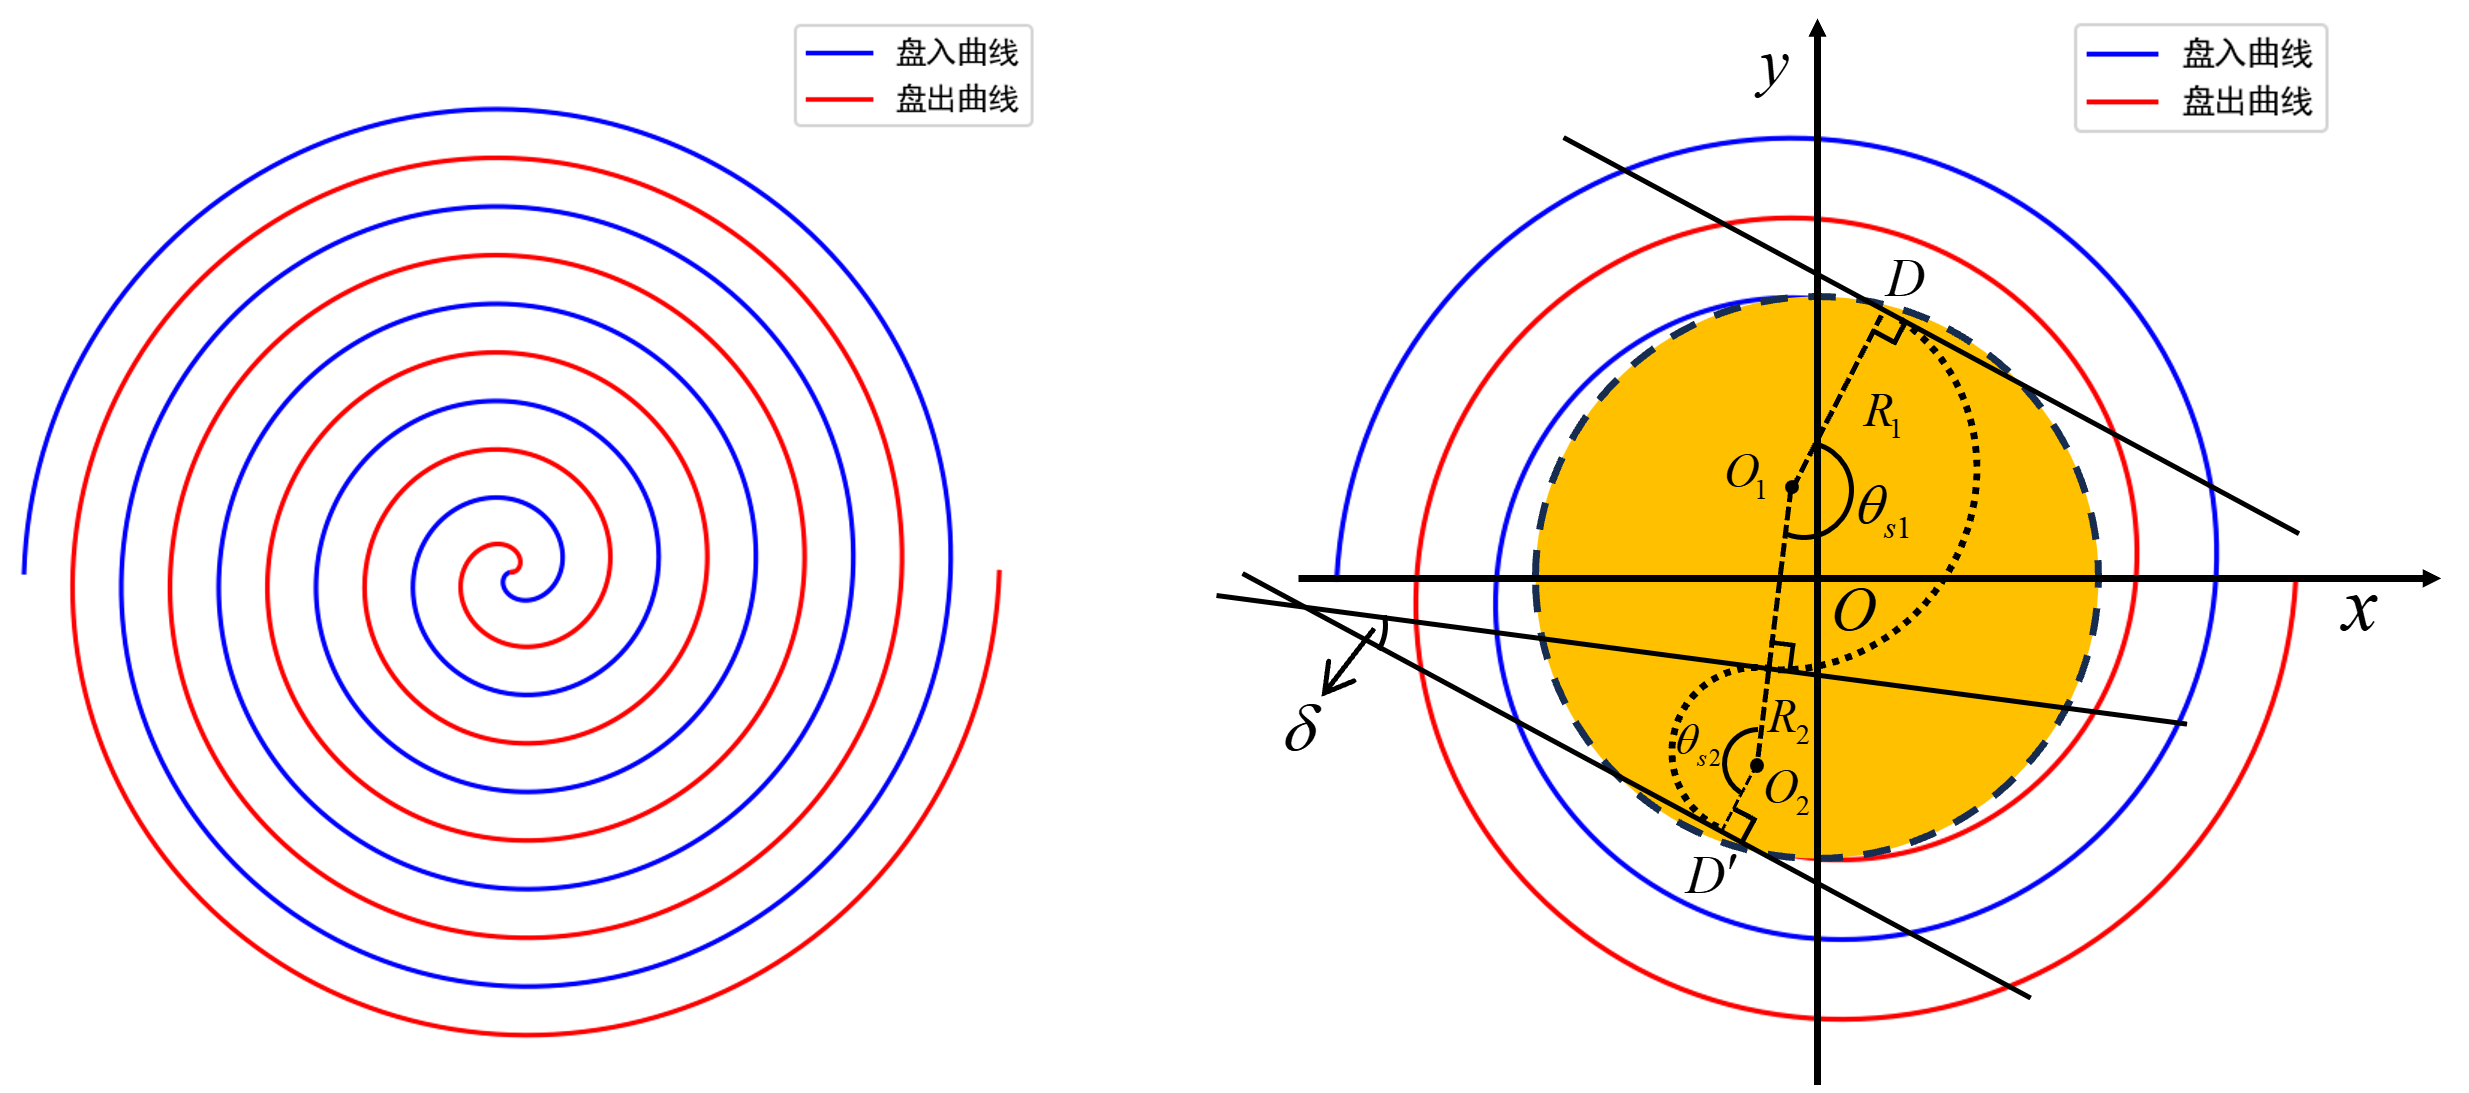
\includegraphics[width=.8\textwidth]{问题四.png}
		\caption{盘入盘出曲线和调头曲线几何关系示意图}
		\label{问题四}
	\end{figure}
	对于调头曲线,由盘入曲线和盘出曲线成中心对称的几何关系与题设可知:
	\begin{equation}
		\begin{cases}
			R_1=2R_2=R\\
			\theta_{s1}=\theta_{s2}=\theta
		\end{cases}
	\end{equation}
	
	调头曲线由两段圆弧组成,其长度可表示为:
	\begin{equation}
		s=\theta_{s1}R_1+\theta_{s2}R_2
	\end{equation}
	
	\textbf{2.最短调头曲线优化模型}
	
	在第四问中舞龙队需要在直径为9m的圆内完成调头,可以证明调头曲线的长度仅与调头点坐标有关:
	设调头点坐标为$D(x_m,y_m)$,盘出调头空间的坐标由中心对称可得$D'(-x_m,-y_m)$。设于圆弧$O_1(x_1,y_1)$、$O_2(x_2,y_2)$相切的直线斜率分别为$k_1$、$k_2$,两圆弧公切线的斜率为$k_3$,如图\ref{问题四}(右)所示。
	
	其中,直线$O_1D$、直线$O_2D'$的方程可表示为:
	\begin{equation}
		\begin{cases}
			\vspace{\topsep}
			y_{O_1 D}=-\dfrac{1}{k_1}(x-x_m)+y_m \\
			y_{O_2 D'}=-\dfrac{1}{k_2}(x+x_m)-y_m
		\end{cases}
	\end{equation}
	
	由几何关系可得:
	\begin{equation}
		\begin{cases}
		O_1 D=2O_2D'\\
		O_1O_2=O_1D+O_2D'
		\end{cases}
	\end{equation}
	
	用代数方程可表示为:
	\begin{equation}
	\begin{cases}
		\vspace{\topsep}
		\delta=tan^{-1}k_3-tan^{-1}k2\\
		\vspace{\topsep}
			y_1=-\dfrac{1}{k_1}(x_1-x_m)+y_m \\
			\vspace{\topsep}
			y_2=-\dfrac{1}{k_2}(x_2+x_m)-y_m \\
			\vspace{\topsep}
		\sqrt{1+(\frac{1}{k_1})^2}|x_m-x_1|=2\sqrt{1+(\frac{1}{k_2})^2}|-x_m-x_2|\\
		\sqrt{(x_1-x_2)^2+(y_1-y_2)^2}=\sqrt{1+(\frac{1}{k_1})^2}|x_m-x_1|+\sqrt{1+(\frac{1}{k_2})^2 }|-x_m-x_2 |
		\end{cases}
	\end{equation}

	由式(32)可得圆弧运动的半径$R$和角度$\theta$为:
	\begin{equation}
		\begin{cases}
			R=\dfrac{1}{3}\sqrt{(x_1-x_2)^2+(y_1-y_2)^2}\\
			\theta=\pi-\delta
		\end{cases}
	\end{equation}
	舞龙队龙头沿螺线盘旋越接近螺线中心所需调头曲线长度越短,使用问题二碰撞模型模拟舞龙队在螺距1.7m的螺线上的运动,发现在盘出时龙头与龙身发生碰撞。因此当舞龙队从最晚调头点调头时恰好能顺利盘出(不发生碰撞),并且此时调头曲线最短。以最晚调头点到原点的距离为半径,原点为圆心作圆,此区域为最小调头空间。
	
	\textbf{3.舞龙队在圆弧曲线上的运动模型}
	
	\textbf{1)位置坐标模型}
	
	板凳在调头圆弧曲线上运动状态如图\ref{扇形}所示:
	\begin{figure}[H]
		\centering
		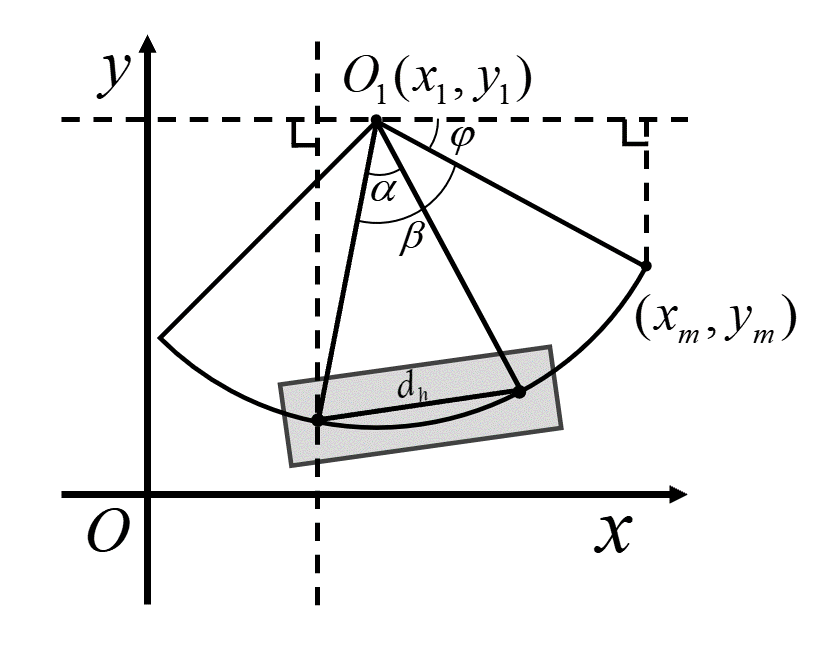
\includegraphics[width=.4\textwidth]{扇形.png}
		\caption{板凳在调头圆弧曲线上运动状态示意图}
		\label{扇形}
	\end{figure}
	
	在圆弧上龙头以匀速运动,以下推导以前部分圆弧为例,则此时龙头的角速度$\omega_h$为:
	\begin{equation}
		\omega_h=\dfrac{v_h}{R_1}
	\end{equation}
	
	以调头时刻为零时刻,龙头从进入圆弧后沿圆心转过的角度$\beta_h$与时间$t$的关系为:
	\begin{equation}
		\beta_h=\omega_ht
	\end{equation}
	
	调头点与圆心连线与$x$轴夹角为:
	\begin{equation}
		\varphi=tan^{-1}(\dfrac{y_1-y_m}{x_m-x_1})
	\end{equation}
	其中,相邻两把手的节点与圆心连线夹角可由余弦定理求得,表示为:
	\begin{equation}
		\begin{cases}
			\vspace{\topsep}
			\alpha_h=cos^{-1}(\dfrac{2R_1^2-d^2_h}{2R_1^2})\mbox{,龙头板凳}\\
			\alpha_b=cos^{-1}(\dfrac{2R_1^2-d^2_b}{2R_1^2})\mbox{,龙身板凳}
		\end{cases}
	\end{equation}
	
	由式(34)(35)(36)可求得龙头前把手的坐标\cite{3},即:
	\begin{equation}
		\begin{cases}
			x_h=x_1+R_1cos(\beta_h+\varphi)\\
			y_h=y_1-R_1sin(\beta_h+\varphi)
		\end{cases}
	\end{equation}
	
	龙头后第$i+1$节龙身前把手坐标可表示为:
	\begin{equation}
		\begin{cases}
			x_{bi}=x_1+R_1cos(\beta_h+\varphi-\alpha_h-i\alpha_b)\\
			y_{bi}=y_1-R_1sin(\beta_h+\varphi-\alpha_h-i\alpha_b)
		\end{cases}
	\end{equation}
	
	\textbf{2)速度模型}
	
	当板凳沿圆弧运动时速度时刻相等,即:
	\begin{equation}
		v_{bi}=v_{b(i+1)}
	\end{equation}
	
	\textbf{4.板凳运动状态的判断}
	
	由调头点坐标可求得板凳从螺线运动进入圆弧运动的临界旋转角,即:
	\begin{equation}
		\theta_{turn}=\dfrac{\sqrt{x_1^2+y_1^2}}{b}
	\end{equation}
	
	根据问题四步长$\Delta t=1s$判断,当$t$时刻满足$\theta \le \theta_{turn}$时表示从该时刻板凳从沿螺线运动转变为沿圆弧运动。
	
	任一板凳从开始圆弧运动到结束时运动的时间可表示为:
	\begin{equation}
		T_i=\dfrac{s}{v_{bi}}
	\end{equation}
	其中,$T_i$、$v_{bi}$分别表示龙头后第$i$节龙身圆弧运动持续的时间和速度。
	\subsubsection{模型求解}
	\textbf{1.最短调头曲线的求解 }
	
	采用问题三所示的调头空间时,将调头空间半径$r_d=4.5$m代入模型可得:
	\begin{equation}
		s=14.854167\mbox{m}
	\end{equation}
	
	对于最短调头曲线的求解,使用二分法和变步长遍历算法寻找调头曲线最小值的流程如下:
	
	\textbf{Step1:}设置调头空间半径的遍历范围$r_d\in[0,4.5]$,取较大的遍历步长$\Delta  r_d=0.1$,遍历,模糊检测到使舞龙队恰好不发生碰撞时$r_d$的取值区间;
	
	\textbf{Step2:}根据得到的取值区间,利用二分法进行$n_0$次迭代,当步长之差小于0.01m时跳出循环,找到准确的$r_d$;
	
	经过二分法求解之后,得到最小调头空间半径$r_d=2.89$m时,在盘入盘出过程中舞龙队恰好不会相撞。进而计算最短调头曲线长度为:
	\begin{equation}
		s_{min}=9.879203\mbox{m}
	\end{equation}
	
	\textbf{2.舞龙队位置和行进速度的求解}
	
	联立调头区域边界方程和盘入曲线方程:
	\begin{equation}
		\begin{cases}
			x^2+y^2=4.5^2\\
			r=b\theta
		\end{cases}
	\end{equation}
	得到调头点坐标$(x_m,y_m)$,该点为零时刻龙头前把手初始坐标。根据临界旋转角度判断板凳运动状态,当在圆弧上运动时,龙身运动状态模型如式(46):
	\begin{equation}
		\begin{cases}
			x_{bi}=x_1+R_1cos(\beta_h+\varphi-\alpha_h-i\alpha_b)\\
			y_{bi}=y_1-R_1sin(\beta_h+\varphi-\alpha_h-i\alpha_b)\\
			v_{bi,(t+1)}=v_{bi,t}
		\end{cases}
	\end{equation}
	其中,$v_{bi,(t+1)}$表示$v_{bi,t}$下一秒运动速度。
	
	在盘入螺线上运动时,由问题一建立的模型得:
	\begin{equation}
		\begin{cases}
			x_{bi}=r_icos\theta_i\\
			y_{bi}=r_isin\theta_i\\
			\dfrac{v_{b(i+1)}}{v_{bi}}=\dfrac{cos\alpha_{(i+1)}}{cos\beta_i}
		\end{cases}
	\end{equation}
	
	龙头前把手的行进速度始终保持 1 m/s。以调头开始时间为零时刻,通过递推求出从−100 s 开始
	到100 s 为止,每秒整个舞龙队的位置和速度,下述表\ref{问题四位置}和表\ref{问题四速度}分别为−100 s、 −50 s、 0 s、 50 s、 100 s 时,龙头前把手、龙头后面第 1、51、101、151、201 节龙身前把手和龙尾后把手的位置和速度,具体求解结果见文件 result4.xlsx。
	\begin{table}[H]
		\centering
		\setlength{\tabcolsep}{9pt}
		\caption{问题四舞龙队的位置} 
		\label{问题四位置} 
		\setlength\extrarowheight{-3pt}
		\small
		\begin{tabular}{|c|c|c|c|c|c|c|}
			\hline
			& -100s& -50s & 0s & 50s & 100s \\ \hline
			龙头x(m) &7.866065 &6.664626&-2.943078&-1.783076&2.746366 \\ \hline
			龙头y(m) & 3.509739& 1.649141 &-3.379179&-6.039617&-7.692214 \\ \hline
			第1节龙身x(m)&6.360066& 5.519350 &-0.375026&4.204898&0.088367\\ \hline
			第1节龙身y(m)& 5.941111& 4.269818& -4.638033&4.518307&8.071554\\ \hline
			第51节龙身x(m) & -10.542447&-3.862677& 2.157886&-1.269492 &2.458889 \\ \hline
			第51节龙身y(m) & 3.046781&-8.858199&-7.856570& -6.191475&3.791881 \\ \hline
			第101节龙身x(m)& -12.000535&9.988706&3.303470&-7.829261 &-6.992109  \\ \hline
			第101节龙身y(m)& -4.591356&-6.187642&10.007598&4.832164&2.836937  \\ \hline
			第151节龙身x(m)& -14.375875&12.895695&-6.739031&-4.224519&9.120762  \\ \hline
			第151节龙身y(m)& -1.757570&-4.053001& 10.503309& -10.558235&-4.293867  \\ \hline
			第201节龙身x(m)&-11.800121&10.335096&-6.596106 &0.754248&9.078184  \\ \hline
			第201节龙身y(m)&10.731721 &-10.980500&12.525488& -13.168898&7.992703  \\ \hline
			龙尾(后)x(m)& -1.234909& 0.444688&-2.241075&5.481340&-11.376227 \\ \hline
			龙尾(后)y(m)&-16.508675 &15.711052 &-14.663702&12.790419&-6.044073 \\ \hline
		\end{tabular}
	\end{table}
	\begin{table}[H]
		\centering
		\setlength{\tabcolsep}{12pt}
		\caption{问题四舞龙队的速度} 
		\label{问题四速度} 
		\setlength\extrarowheight{-3pt}
		\small
		\begin{tabular}{|c|c|c|c|c|c|c|}
			\hline
			& -100s& -50s & 0s & 50s & 100s \\ \hline
			龙头(m/s) &1.000000 &1.000000 &1.000000 &1.000000 &1.000000  \\ \hline
			第1节龙身(m/s) & 0.999904&0.999761& 0.998664& 1.000368&1.000125  \\ \hline
			第51节龙身(m/s) &0.999344& 0.998635& 0.995074& 0.999998&1.004026  \\ \hline
			第101节龙身(m/s) &0.999089& 0.998241& 0.994385& 0.998482&1.000330    \\ \hline
			第151节龙身(m/s) &0.998942&0.998039& 0.994092& 0.998017&0.999446    \\ \hline
			第201节龙身(m/s) &0.998847&0.997917& 0.993930& 0.997791&0.999103   \\ \hline
			龙尾(后)(m/s) &0.998815&0.997877 & 0.993880& 0.997725&0.999011   \\ \hline
		\end{tabular}
	\end{table}
	\subsection{问题五的模型建立与求解}
	\subsubsection{舞龙队运动速度分析}
	舞龙队在设定的路径中共有三段不同运动轨迹:沿等距螺线盘入轨迹$P_1$,在调头区域中沿S型圆弧调头曲线运动轨迹$P_2$、与盘入曲线中心对称的盘出曲线$P_3$。
	在$P_1$上由问题一所求解数据可知:盘入螺线时,舞龙队中龙头速度最大,龙身速度逐节递减;$P_2$上的运动为标准圆周运动,各节板凳的运动速度相等;$P_3$为盘出曲线,为与盘入曲线相位相差为$\pi$的等距落线,舞龙队在$P_3$上的运动规律与$P_1$类似,其中龙头速度最小,龙身速度逐节递增。
	\subsubsection{龙头最大行进速度模型求解}
	由题目条件得,舞龙队各把手的速度均不超过2m/s,可确定约束条件为:
	\begin{equation}
		\mbox{max}\{v_h,v_{bi}\}\le 2\mbox{m/s}
	\end{equation}
	
	舞龙队在设定路径中行进时,由5.5.1分析可知龙尾后把手恰好进入盘出曲线时的速度即为舞龙队运动过程中的最大行进速度,使用二分法求解龙头速度不同时的龙尾速度,找到最大速度刚好小于2m/s时龙头的速度。计算龙头在约束条件下的最大行进速度为:
	\begin{equation}
		v_{h\_max}=1.989837\mbox{m/s}
	\end{equation}
	\section{灵敏度分析}
	在问题三中,调头空间为一直径恒定的圆,求解了最小螺距使舞龙队能够顺利盘入调头区域。为了探究调头空间圆半径$r_d$的取值对最小螺距$d_{min}$的影响,让调头空间半径$r_d$在[2.5,5.5]之间以$r_d=0.2$的步长变化,研究最小螺距$d_{min}$的变化程度,得到了最小螺距随调头空间圆半径$r_d$变化的折线(左)和其一阶差分折线(右)如图\ref{分析}。
	\begin{figure}[H]
		\centering
		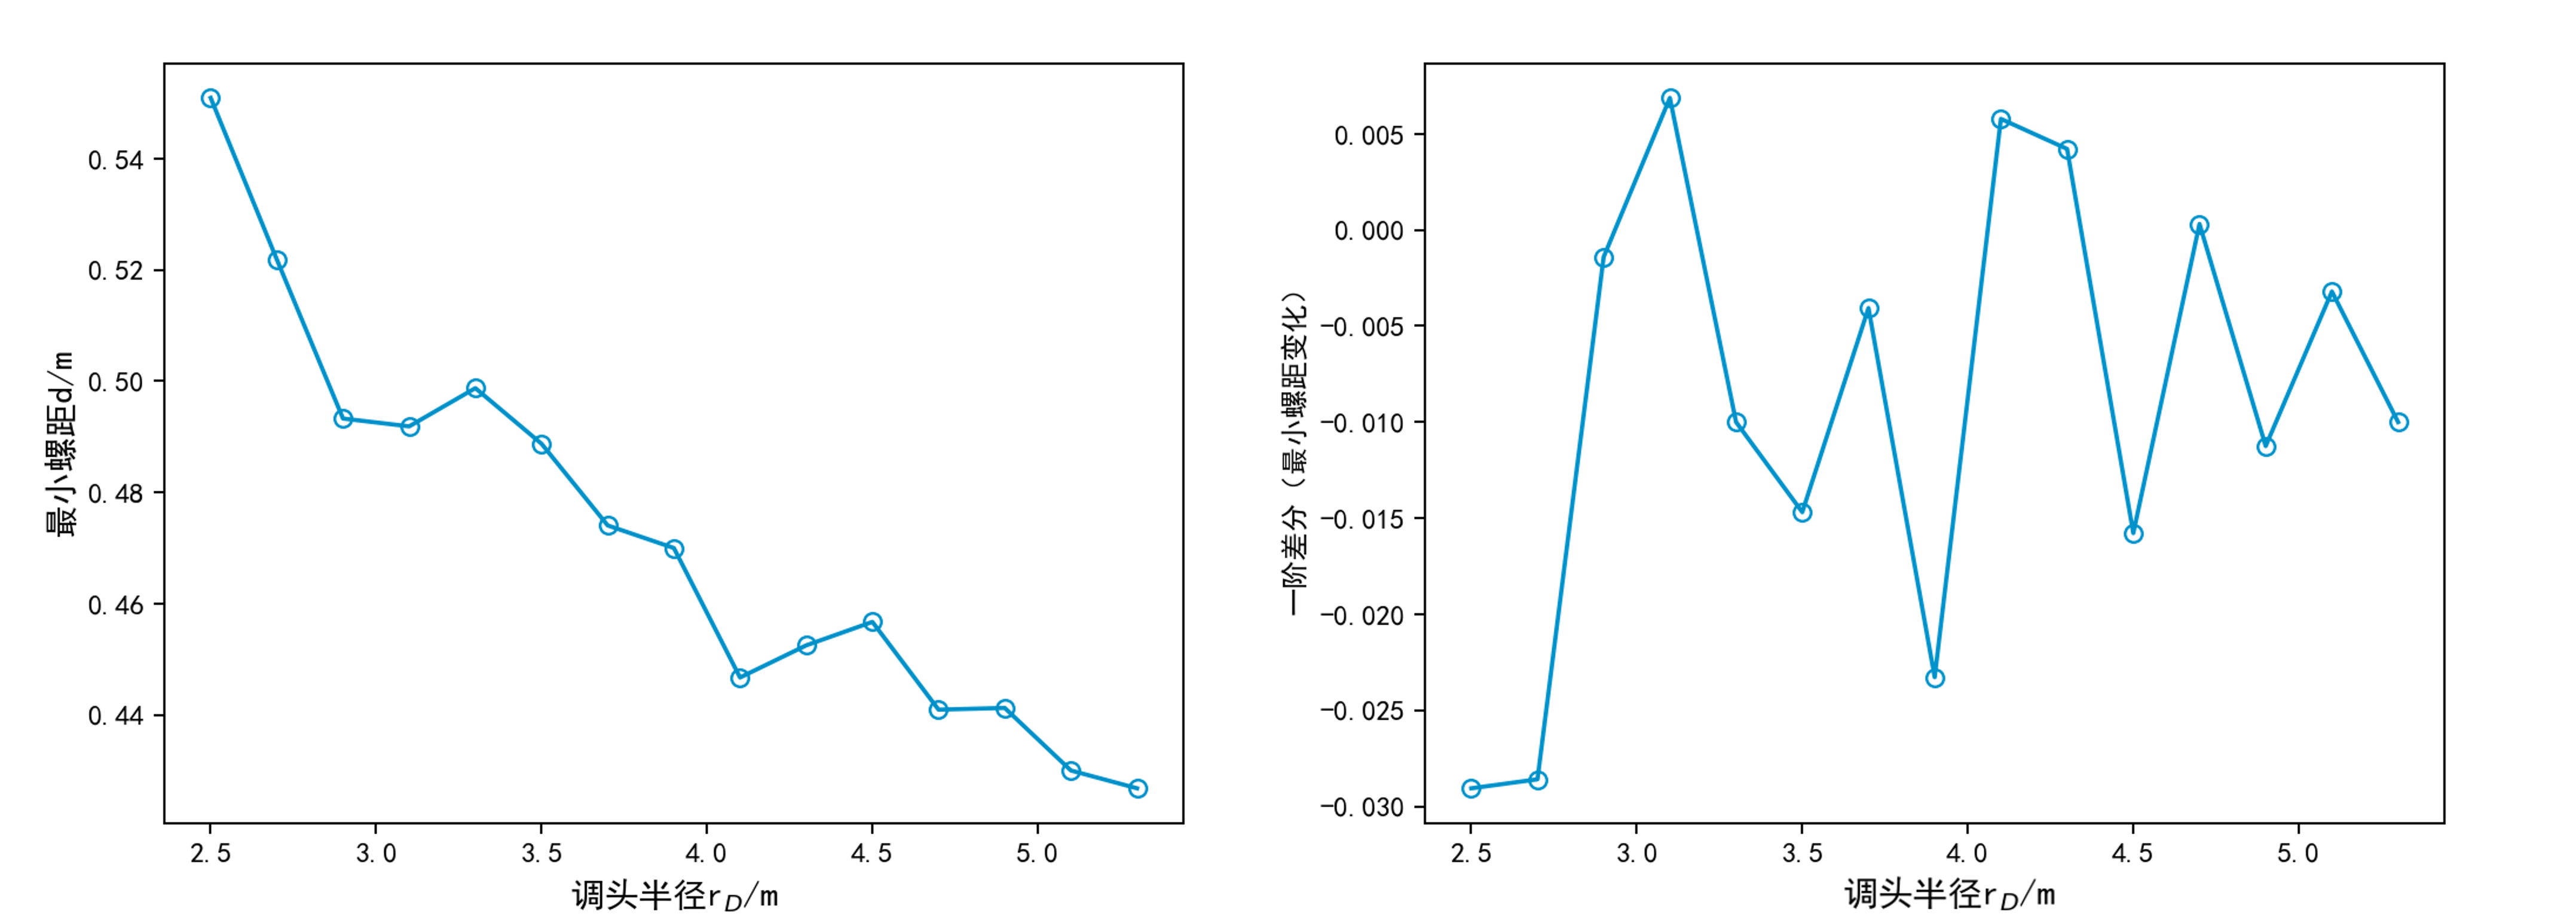
\includegraphics[width=1.0\textwidth]{灵敏度分析.png}
		\caption{最小螺距随调头空间圆半径变化和其一阶差分折线图}
		\label{分析}
	\end{figure}
	从图\ref{分析}左中可已看出随着调头半径的增大,最小螺距整体呈减小趋势,调头空间半径在区间内变化幅度约为17\%,且由一阶差分折线图\ref{分析}右可以发现最小螺距在调头半径区间[4.7,5.5]逐渐趋于平稳。
	一般来说,在舞龙队可灵活盘入和盘出的前提下,缩小盘龙所需的面积,增加盘龙行进速度,即可提高观赏性。螺距越小盘龙所需面积越小,考虑到上述灵敏度分析,在问题三实际情况中在[4.7,5.0]中选择调头空间半径最优。
	\section{模型的评价}
	
	\subsection{模型的优点}
	1.问题一和问题二求解速度时考虑到同一板凳上两把手沿板方向上速度分量相等的物理关系简化了速度求解过程;
	
	2.问题三遍历求解最小螺距时引入二分法的思想降低了时间复杂度;
	
	3.问题四中通过模拟舞龙队盘出运动找到了更小的调头空间和调头曲线。
	
	
	\subsection{模型的缺点}
	1.在判断碰撞时,需要考虑每一节板凳四个顶点与其他非相邻板凳的位置状态,计算量较大且繁杂,使得求解时间较长;
	
	2.求解更短的调头曲线时仅考虑盘入点与盘出点中心对称的情况,可能导致求解结果不是最短曲线长度,存在可接受误差。
	\section{模型的改进与推广}
	1.考虑舞龙队发生碰撞的三维空间模型,使结果更贴合实际情况;
	
	2.提高二分法迭代次数,使用更小步长遍历,提高结果精确度;
	
	3.本论文所建立的运动模型可以应用于运动轨迹为阿基米德螺线的物理问题。
	
	
	\begin{thebibliography}{9}%宽度9
		\bibitem[1]{1}
		孙森震,卢小平,武永斌,等.
		\newblock 基于阿基米德螺线的地铁隧道建模方法\allowbreak[J].
		\newblock 测绘通报,2015,(04):72-74+121.DOI:10.13474/j.cnki.11-2246.2015.0114.
		
		\bibitem[2]{2}
		罗良玲,曹苏明.
		\newblock 基于时间分割法的阿基米德螺线的插补算法研究\allowbreak[J].
		\newblock 南昌大学学报(工科版),2002,(03):22-24.
		
		\bibitem[3]{3}
		闫敏,刘涛,麻德权,等.
		\newblock 利用代数-阿基米德双螺线构建变截面涡旋齿组合型线\allowbreak[J].
		\newblock 上海交通大学学报,2024,58(08):1282-1289.DOI:10.16183/j.cnki.jsjtu.2022.532.
		
	%	\bibitem[1]{海洋能}
	%	王振春,王年果,栾锋.
	%	\newblock 波浪能转换装置主动控制研究现状与发展\allowbreak[J].
	%	\newblock 燕山大学学报,2023,47(03):189-199.
	%	\bibitem[2]{平行轴定理}
	%	维基百科.
	%	\newblock https://zh.wikipedia.org/wiki/平行轴定理

	\end{thebibliography}
	\newpage
	%附录
	\section*{附录}
	\appendix
	\section{\quad 支撑材料文件列表}
	\subsection*{·问题一}
	result1.xlsx——题目要求结果
	
	Question1.py——求解问题一的程序
	\subsection*{·问题二}
	result2.xlsx——题目要求结果
	
	Question2.py——求解问题二的程序
	\subsection*{·问题三}
	Question3.py——求解问题三的程序
	
	灵敏度分析.py——探究调头空间圆的半径对最小螺距的影响
	\subsection*{·问题四}
	result4.xlsx——题目要求结果
	
	Question4.py——求解问题四的程序
	\subsection*{·问题五}
	Question5.py——求解问题五的程序
	\subsection*{·论文相关材料}
	2024A.tex——撰写论文的Tex代码
	\section{\quad 源代码}
	\subsubsection*{Question1.py}
	\begin{lstlisting}[language=Python]
	import numpy as np
	import pandas as pd
	#参数
	n=223
	b=0.55
	pi=np.pi
	t_max=301
	v_h=1
	d_h=2.86
	d_b=1.65
	
	#计算每一时刻龙头位置
	def theta(t):
	theta=np.sqrt(-4*pi*v_h*t/b+1024*pi*pi)
	return theta
	
	theta_head=[]
	r_head=[]
	head_x=[]
	head_y=[]
	for t in range(t_max+1):
	theta_now=theta(t)
	theta_head.append(theta_now)
	r_head.append(b*theta_now/(2*pi))
	x=r_head[t]*np.cos(theta_now)
	y=r_head[t]*np.sin(theta_now)
	x=round(x,6)
	y=round(y,6)
	head_x.append(x)
	head_y.append(y)
	
	#牛顿法解方程,求解各点的位置
	def f(theta_now,theta_next,d):
	return (b*b/4/pi/pi)*(theta_now**2+theta_next**2-2*theta_now*theta_next*
	np.cos(theta_now-theta_next))-d**2
	def f_prime(theta_now,theta_next,d):
	return (b*b/4/pi/pi)*(2*theta_next+2*theta_now*(np.cos(theta_now-theta_next)-
	theta_next*np.sin(theta_now-theta_next)))
	
	def newton_method(f,f_prime,d,theta_now,x0,tol=1e-6,max_iter=100):
	for i in range(max_iter):
	x = x0 - f(theta_now,x0,d) / f_prime(theta_now,x0,d)
	if abs(x - x0) < tol:
	break
	x0 = x
	return x
	
	theta_body_i=np.empty((n,t_max+1))
	r_body_i=np.empty((n,t_max+1))
	body_i_x=np.empty((n,t_max+1))
	body_i_y=np.empty((n,t_max+1))
	for t in range(t_max+1):
	theta_next=newton_method(f,f_prime,d_h,theta_head[t],theta_head[t]+pi/2)
	theta_body_i[0][t]=theta_next
	r_body_i[0][t]=theta_next*b/(2*pi)
	x=r_body_i[0][t]*np.cos(theta_next)
	y=r_body_i[0][t]*np.sin(theta_next)
	x=round(x,6)
	y=round(y,6)
	body_i_x[0][t]=x
	body_i_y[0][t]=y
	
	for i in range(1,n):
	for t in range(t_max+1):
	theta_next=newton_method(f,f_prime,d_b,theta_body_i[i-1][t],theta_body_i[i-1][t]+pi/2)
	theta_body_i[i][t]=theta_next
	r_body_i[i][t]=theta_next*b/(2*pi)
	x=r_body_i[i][t]*np.cos(theta_next)
	y=r_body_i[i][t]*np.sin(theta_next)
	x=round(x,6)
	y=round(y,6)
	body_i_x[i][t]=x
	body_i_y[i][t]=y
	
	#求解各点速度
	v_body_i=np.empty((n,t_max+1))
	for t in range(t_max):
	m_0=(head_y[t]-body_i_y[0][t])/(head_x[t]-body_i_x[0][t])
	m_now=(theta_head[t]*np.cos(theta_head[t])+np.sin(theta_head[t]))/
	(-theta_head[t]*np.sin(theta_head[t])+np.cos(theta_head[t]))
	m_next=(theta_body_i[0][t]*np.cos(theta_body_i[0][t])+np.sin(theta_body_i[0][t]))/
	(-theta_body_i[0][t]*np.sin(theta_body_i[0][t])+np.cos(theta_body_i[0][t]))
	alpha_1=np.arctan(np.abs((m_0-m_now)/(1+m_0*m_now)))
	alpha_2=np.arctan(np.abs((m_0-m_next)/(1+m_0*m_next)))
	v_next=v_h*np.cos(alpha_1)/np.cos(alpha_2)
	v_next=round(v_next,6)
	v_body_i[0][t]=v_next
	
	for i in range(1,n):
	for t in range(t_max):
	m_0=(body_i_y[i][t]-body_i_y[i-1][t])/(body_i_x[i][t]-body_i_x[i-1][t])
	m_now=(theta_body_i[i-1][t]*np.cos(theta_body_i[i-1][t])+np.sin(theta_body_i[i-1][t]))/
	(-theta_body_i[i-1][t]*np.sin(theta_body_i[i-1][t])+np.cos(theta_body_i[i-1][t]))
	m_next=(theta_body_i[i][t]*np.cos(theta_body_i[i][t])+np.sin(theta_body_i[i][t]))/
	(-theta_body_i[i][t]*np.sin(theta_body_i[i][t])+np.cos(theta_body_i[i][t]))
	alpha_1=np.arctan(np.abs((m_0-m_now)/(1+m_0*m_now)))
	alpha_2=np.arctan(np.abs((m_0-m_next)/(1+m_0*m_next)))
	v_next=v_body_i[i-1][t]*np.cos(alpha_1)/np.cos(alpha_2)
	v_next=round(v_next,6)
	v_body_i[i][t]=v_next
	
	#输出固定时间,固定位置的位置速度
	time_point=[0,60,120,180,240,300]
	num_point=[0,50,100,150,200,222]
	
	for t in time_point:
	print(f"time:{t}")
	print(f"head:x:{head_x[t]},y:{head_y[t]},v:{v_h}")
	for i in num_point:
	print(f"body{i}:x:{body_i_x[i][t]},y:{body_i_y[i][t]},v:{v_body_i[i][t]}")
	
	#将结果写入excel
	data=[]
	data.append(head_x)
	data.append(head_y)
	for i in range(n):
	data.append(body_i_x[i])
	data.append(body_i_y[i])
	df=pd.DataFrame(data)
	df.to_excel('solution1-1.xlsx')
	
	data_v=v_body_i
	df=pd.DataFrame(data_v)
	df.to_excel('solution1-2.xlsx')
	\end{lstlisting}
	\subsubsection*{Question2.py}
	\begin{lstlisting}[language=Python]
	import numpy as np
	import pandas as pd
	#参数
	n=223
	b=0.55
	pi=np.pi
	t_max=300
	v_h=1
	d_h=2.86
	d_b=1.65
	l_h=3.41
	l_b=2.2
	
	#计算每一时刻龙头位置
	def theta(t):
	theta=np.sqrt(-4*pi*v_h*t/b+1024*pi*pi)
	return theta
	
	#牛顿法解方程,求解各点的位置
	def f(theta_now,theta_next,d):
	return (b*b/4/pi/pi)*(theta_now**2+theta_next**2-2*theta_now*theta_next*
	np.cos(theta_now-theta_next))-d**2
	def f_prime(theta_now,theta_next,d):
	return (b*b/4/pi/pi)*(2*theta_next+2*theta_now*(np.cos(theta_now-theta_next)-
	theta_next*np.sin(theta_now-theta_next)))
	
	def newton_method(f,f_prime,d,theta_now,x0,tol=1e-6,max_iter=100):
	for i in range(max_iter):
	x = x0 - f(theta_now,x0,d) / f_prime(theta_now,x0,d)
	if abs(x - x0) < tol:
	break
	x0 = x
	return x
	
	#考虑矩形的4个角
	def corner(x1,y1,x2,y2,l):
	k=(y2-y1)/(x2-x1)
	k_p=-1/k
	db=np.sqrt(1+k**2)*0.15
	b_0=(x1*y2-x2*y1)/(x1-x2)
	b_1=b_0-db
	b_2=b_0+db
	mid_x=(x1+x2)/2
	mid_y=(y1+y2)/2
	c_0=mid_y-k_p*mid_x
	dc=np.sqrt(1+k_p**2)*(l/2)
	c_1=c_0-dc
	c_2=c_0+dc
	x_a=(c_1-b_1)/(k-k_p)
	y_a=k*x_a+b_1
	x_b=(c_1-b_2)/(k-k_p)
	y_b=k*x_b+b_2
	x_c=(c_2-b_1)/(k-k_p)
	y_c=k*x_c+b_1
	x_d=(c_2-b_2)/(k-k_p)
	y_d=k*x_d+b_2
	return x_a,y_a,x_b,y_b,x_c,y_c,x_d,y_d
	
	#判断点是否在矩形内
	def is_in_rectangle(x,y,x1,y1,x2,y2,l):
	k=(y2-y1)/(x2-x1)
	b=(x1*y2-x2*y1)/(x1-x2)
	d=np.abs(k*x-y+b)/np.sqrt(1+k**2)
	if d>0.15:
	return False
	else:
	x0=(k*(y-b)+x)/(1+k**2)
	dis_sum=(1+k**2)*(np.abs(x1-x0)+np.abs(x2-x0))
	if dis_sum>l:
	return False
	else:
	return True
	
	theta_head=[]
	r_head=[]
	head_x=[]
	head_y=[]
	theta_body_i=np.empty((n,2*t_max))
	r_body_i=np.empty((n,2*t_max))
	body_i_x=np.empty((n,2*t_max))
	body_i_y=np.empty((n,2*t_max))
	t=0
	flag=False
	while flag==False:
	#计算龙头位置
	theta_now=theta(t)
	theta_head.append(theta_now)
	r_head.append(b*theta_now/(2*pi))
	x=r_head[t]*np.cos(theta_now)
	y=r_head[t]*np.sin(theta_now)
	x=round(x,6)
	y=round(y,6)
	head_x.append(x)
	head_y.append(y)
	#计算下一节位置
	theta_next=newton_method(f,f_prime,d_h,theta_head[t],theta_head[t]+pi/2)
	theta_body_i[0][t]=theta_next
	r_body_i[0][t]=theta_next*b/(2*pi)
	x=r_body_i[0][t]*np.cos(theta_next)
	y=r_body_i[0][t]*np.sin(theta_next)
	x=round(x,6)
	y=round(y,6)
	body_i_x[0][t]=x
	body_i_y[0][t]=y
	for i in range(1,n):
	theta_next=newton_method(f,f_prime,d_b,theta_body_i[i-1][t],theta_body_i[i-1][t]+pi/2)
	theta_body_i[i][t]=theta_next
	r_body_i[i][t]=theta_next*b/(2*pi)
	x=r_body_i[i][t]*np.cos(theta_next)
	y=r_body_i[i][t]*np.sin(theta_next)
	x=round(x,6)
	y=round(y,6)
	body_i_x[i][t]=x
	body_i_y[i][t]=y
	#判断是否与龙头碰撞
	x1=head_x[t]
	y1=head_y[t]
	x2=body_i_x[0][t]
	y2=body_i_y[0][t]
	x_a,y_a,x_b,y_b,x_c,y_c,x_d,y_d=corner(x1,y1,x2,y2,l_h)
	for i in range(1,n-1):
	if(is_in_rectangle(x_a,y_a,body_i_x[i][t],
	body_i_y[i][t],body_i_x[i+1][t],body_i_y[i+1][t],l_h)):
	print(f"在t={t}时刻,龙头和第{i+1}个板子碰撞")
	flag=True
	break
	elif(is_in_rectangle(x_b,y_b,body_i_x[i][t],
	body_i_y[i][t],body_i_x[i+1][t],body_i_y[i+1][t],l_h)):
	print(f"在t={t}时刻,龙头和第{i+1}个板子碰撞")
	flag=True
	break
	elif(is_in_rectangle(x_c,y_c,body_i_x[i][t],
	body_i_y[i][t],body_i_x[i+1][t],body_i_y[i+1][t],l_h)):
	print(f"在t={t}时刻,龙头和第{i+1}个板子碰撞")
	flag=True
	break
	elif(is_in_rectangle(x_d,y_d,body_i_x[i][t],
	body_i_y[i][t],body_i_x[i+1][t],body_i_y[i+1][t],l_h)):
	print(f"在t={t}时刻,龙头和第{i+1}个板子碰撞")
	flag=True
	break
	
	#判断是否与龙身碰撞
	for i in range(0,n-1):
	x1=body_i_x[i][t]
	y1=body_i_y[i][t]
	x2=body_i_x[i+1][t]
	y2=body_i_y[i+1][t]
	x_a,y_a,x_b,y_b,x_c,y_c,x_d,y_d=corner(x1,y1,x2,y2,l_b)
	for j in range(i+2,n-1):
	if(is_in_rectangle(x_a,y_a,body_i_x[j][t],body_i_y[j][t],
	body_i_x[j+1][t],body_i_y[j+1][t],l_b)):
	print(f"在t={t}时刻,第{i}块板子和第{j+1}个板子碰撞")
	flag=True
	break
	elif(is_in_rectangle(x_b,y_b,body_i_x[j][t],body_i_y[j][t],
	body_i_x[j+1][t],body_i_y[j+1][t],l_b)):
	print(f"在t={t}时刻,第{i}块板子和第{j+1}个板子碰撞")
	flag=True
	break
	elif(is_in_rectangle(x_c,y_c,body_i_x[j][t],body_i_y[j][t],
	body_i_x[j+1][t],body_i_y[j+1][t],l_b)):
	print(f"在t={t}时刻,第{i}块板子和第{j+1}个板子碰撞")
	flag=True
	break
	elif(is_in_rectangle(x_d,y_d,body_i_x[j][t],body_i_y[j][t],
	body_i_x[j+1][t],body_i_y[j+1][t],l_b)):
	print(f"在t={t}时刻,第{i}块板子和第{i+1}个板子碰撞")
	flag=True
	break
	t=t+1
	t=t-1
	#求解该时刻速度
	v_body_i=[]
	m_0=(head_y[t]-body_i_y[0][t])/(head_x[t]-body_i_x[0][t])
	m_now=(theta_head[t]*np.cos(theta_head[t])+np.sin(theta_head[t]))/(-theta_head[t]*
	np.sin(theta_head[t])+np.cos(theta_head[t]))
	m_next=(theta_body_i[0][t]*np.cos(theta_body_i[0][t])+np.sin(theta_body_i[0][t]))/
	(-theta_body_i[0][t]*np.sin(theta_body_i[0][t])+np.cos(theta_body_i[0][t]))
	alpha_1=np.arctan(np.abs((m_0-m_now)/(1+m_0*m_now)))
	alpha_2=np.arctan(np.abs((m_0-m_next)/(1+m_0*m_next)))
	v_next=v_h*np.cos(alpha_1)/np.cos(alpha_2)
	v_next=round(v_next,6)
	v_body_i.append(v_next)
	for i in range(1,n):
	m_0=(body_i_y[i][t]-body_i_y[i-1][t])/(body_i_x[i][t]-body_i_x[i-1][t])
	m_now=(theta_body_i[i-1][t]*np.cos(theta_body_i[i-1][t])+np.sin(theta_body_i[i-1][t]))/
	(-theta_body_i[i-1][t]*np.sin(theta_body_i[i-1][t])+np.cos(theta_body_i[i-1][t]))
	m_next=(theta_body_i[i][t]*np.cos(theta_body_i[i][t])+np.sin(theta_body_i[i][t]))/
	(-theta_body_i[i][t]*np.sin(theta_body_i[i][t])+np.cos(theta_body_i[i][t]))
	alpha_1=np.arctan(np.abs((m_0-m_now)/(1+m_0*m_now)))
	alpha_2=np.arctan(np.abs((m_0-m_next)/(1+m_0*m_next)))
	v_next=v_body_i[i-1]*np.cos(alpha_1)/np.cos(alpha_2)
	v_next=round(v_next,6)
	v_body_i.append(v_next)
	print(f"t={t}时,龙头的位置x={head_x[t]},y={head_y[t]},龙头的速度v={v_h}")
	
	data={
		'x': body_i_x[:,t],
		"y": body_i_y[:,t],
		"v": v_body_i
	}
	df=pd.DataFrame(data)
	df.to_excel("solution2.xlsx")
	
	#打印固定位置的信息
	num_point=[0,50,100,150,200,222]
	print(f"time:{t}")
	print(f"head:x:{head_x[t]},y:{head_y[t]},v:1")
	for i in num_point:
	print(f"body{i}:x:{body_i_x[i][t]},y:{body_i_y[i][t]},v:{v_body_i[i]}")
	\end{lstlisting}
	\subsubsection*{Question3.py}
	\begin{lstlisting}[language=Python]
	import numpy as np
	import pandas as pd
	import matplotlib.pyplot as plt
	np.seterr(divide='ignore',invalid='ignore')
	plt.rcParams['font.sans-serif'] = ['SimHei']
	plt.rcParams['axes.unicode_minus'] = False
	#参数
	n=223
	pi=np.pi
	t_max=300
	v_h=1
	d_h=2.86
	d_b=1.65
	l_h=3.41
	l_b=2.2
	
	#计算每一时刻龙头位置
	def theta(t,b):
	theta=np.sqrt(-4*pi*v_h*t/b+(32*pi*0.55/b)**2)
	return theta
	
	#牛顿法解方程,求解各点的位置
	def f(theta_now,theta_next,d,b):
	return (b*b/4/pi/pi)*(theta_now**2+theta_next**2-2*theta_now*theta_next*
	np.cos(theta_now-theta_next))-d**2
	def f_prime(theta_now,theta_next,d,b):
	return (b*b/4/pi/pi)*(2*theta_next+2*theta_now*(np.cos(theta_now-theta_next)-theta_next*
	np.sin(theta_now-theta_next)))
	
	def newton_method(f,f_prime,d,theta_now,x0,b,tol=1e-6,max_iter=100):
	for i in range(max_iter):
	x = x0 - f(theta_now,x0,d,b) / f_prime(theta_now,x0,d,b)
	if abs(x - x0) < tol:
	break
	x0 = x
	return x    
	
	#考虑矩形的4个角
	def corner(x1,y1,x2,y2,l):
	k=(y2-y1)/(x2-x1)
	k_p=-1/k
	db=np.sqrt(1+k**2)*0.15
	b_0=(x1*y2-x2*y1)/(x1-x2)
	b_1=b_0-db
	b_2=b_0+db
	mid_x=(x1+x2)/2
	mid_y=(y1+y2)/2
	c_0=mid_y-k_p*mid_x
	dc=np.sqrt(1+k_p**2)*(l/2)
	c_1=c_0-dc
	c_2=c_0+dc
	x_a=(c_1-b_1)/(k-k_p)
	y_a=k*x_a+b_1
	x_b=(c_1-b_2)/(k-k_p)
	y_b=k*x_b+b_2
	x_c=(c_2-b_1)/(k-k_p)
	y_c=k*x_c+b_1
	x_d=(c_2-b_2)/(k-k_p)
	y_d=k*x_d+b_2
	return x_a,y_a,x_b,y_b,x_c,y_c,x_d,y_d
	
	#判断点是否在矩形内
	def is_in_rectangle(x,y,x1,y1,x2,y2,l):
	k=(y2-y1)/(x2-x1)
	b=(x1*y2-x2*y1)/(x1-x2)
	d=np.abs(k*x-y+b)/np.sqrt(1+k**2)
	if d>0.15:
	return False
	else:
	x0=(k*(y-b)+x)/(1+k**2)
	dis_sum=(1+k**2)*(np.abs(x1-x0)+np.abs(x2-x0))
	if dis_sum>l:
	return False
	else:
	return True
	
	#计算碰撞时距离
	def dis(b_test):
	theta_head=[]
	r_head=[]
	head_x=[]
	head_y=[]
	theta_body_i=np.empty((n,2*t_max))
	r_body_i=np.empty((n,2*t_max))
	body_i_x=np.empty((n,2*t_max))
	body_i_y=np.empty((n,2*t_max))
	t=0
	flag=False
	while flag==False:
	#计算龙头位置
	theta_now=theta(t,b_test)
	theta_head.append(theta_now)
	r_head.append(b_test*theta_now/(2*pi))
	x=r_head[t]*np.cos(theta_now)
	y=r_head[t]*np.sin(theta_now)
	x=round(x,6)
	y=round(y,6)
	head_x.append(x)
	head_y.append(y)
	#计算下一节位置
	theta_next=newton_method(f,f_prime,d_h,theta_head[t],theta_head[t]+pi/2,b_test)
	theta_body_i[0][t]=theta_next
	r_body_i[0][t]=theta_next*b_test/(2*pi)
	x=r_body_i[0][t]*np.cos(theta_next)
	y=r_body_i[0][t]*np.sin(theta_next)
	x=round(x,6)
	y=round(y,6)
	body_i_x[0][t]=x
	body_i_y[0][t]=y
	for i in range(1,n):
	theta_next=newton_method(f,f_prime,d_b,theta_body_i[i-1][t],theta_body_i[i-1][t]+pi/2,b_test)
	theta_body_i[i][t]=theta_next
	r_body_i[i][t]=theta_next*b_test/(2*pi)
	x=r_body_i[i][t]*np.cos(theta_next)
	y=r_body_i[i][t]*np.sin(theta_next)
	x=round(x,6)
	y=round(y,6)
	body_i_x[i][t]=x
	body_i_y[i][t]=y
	#判断是否与龙头碰撞
	x1=head_x[t]
	y1=head_y[t]
	x2=body_i_x[0][t]
	y2=body_i_y[0][t]
	x_a,y_a,x_b,y_b,x_c,y_c,x_d,y_d=corner(x1,y1,x2,y2,l_h)
	for i in range(1,n-1):
	if(is_in_rectangle(x_a,y_a,body_i_x[i][t],body_i_y[i][t],
	body_i_x[i+1][t],body_i_y[i+1][t],l_h)):
	flag=True
	break
	elif(is_in_rectangle(x_b,y_b,body_i_x[i][t],body_i_y[i][t],
	body_i_x[i+1][t],body_i_y[i+1][t],l_h)):
	flag=True
	break
	elif(is_in_rectangle(x_c,y_c,body_i_x[i][t],body_i_y[i][t],
	body_i_x[i+1][t],body_i_y[i+1][t],l_h)):
	flag=True
	break
	elif(is_in_rectangle(x_d,y_d,body_i_x[i][t],body_i_y[i][t],
	body_i_x[i+1][t],body_i_y[i+1][t],l_h)):
	flag=True
	break
	
	#判断是否与龙身碰撞
	for i in range(0,n-1):
	x1=body_i_x[i][t]
	y1=body_i_y[i][t]
	x2=body_i_x[i+1][t]
	y2=body_i_y[i+1][t]
	x_a,y_a,x_b,y_b,x_c,y_c,x_d,y_d=corner(x1,y1,x2,y2,l_b)
	for j in range(i+2,n-1):
	if(is_in_rectangle(x_a,y_a,body_i_x[j][t],body_i_y[j][t],
	body_i_x[j+1][t],body_i_y[j+1][t],l_b)):
	flag=True
	break
	elif(is_in_rectangle(x_b,y_b,body_i_x[j][t],body_i_y[j][t],
	body_i_x[j+1][t],body_i_y[j+1][t],l_b)):
	flag=True
	break
	elif(is_in_rectangle(x_c,y_c,body_i_x[j][t],body_i_y[j][t],
	body_i_x[j+1][t],body_i_y[j+1][t],l_b)):
	flag=True
	break
	elif(is_in_rectangle(x_d,y_d,body_i_x[j][t],body_i_y[j][t],
	body_i_x[j+1][t],body_i_y[j+1][t],l_b)):
	flag=True
	break
	t=t+1
	t=t-1
	return np.sqrt(head_x[t]**2+head_y[t]**2)
	
	#二分答案
	L=0.4
	R=0.5
	step=0.001
	while L<=R:
	mid=(L+R)/2
	if dis(mid)>4.5:
	L=mid+step
	else:
	R=mid-step
	print(R)
	#遍历
	# b_list=np.arange(0,0.55,0.01)
	# r_list=[]
	# whlie b in b_list:
	#     r_list.append(dis(b))
	# plt.scatter(b_list,r_list)
	# plt.xlabel('螺距d/m')
	# plt.ylabel('碰撞半径r/m')
	# plt.title('碰撞半径随螺距变化的关系')
	# plt.show()
	\end{lstlisting}
	\subsubsection*{Question4.py}
	\begin{lstlisting}[language=Python]
	import numpy as np
	import pandas as pd
	import math
	#参数
	n=223
	b=1.7
	pi=np.pi
	t_max=300
	v_h=1
	d_h=2.86
	d_b=1.65
	l_h=3.41
	l_b=2.2
	R=4.5
	
	#计算盘入每一时刻龙头位置
	def theta(t):
	if -4*pi*v_h*t/b+(32*pi*0.55/b)**2<0:
	return -1
	theta=np.sqrt(-4*pi*v_h*t/b+(32*pi*0.55/b)**2)
	return theta
	
	#计算盘出每一时刻龙头位置
	def theta_out(t):
	theta=np.sqrt(4*pi*v_h*t/b+(2*pi*R/b)**2)
	return theta
	
	#牛顿法解方程,求解各点的位置
	def f(theta_now,theta_next,d):
	return (b*b/4/pi/pi)*(theta_now**2+theta_next**2-2*theta_now*theta_next*
	np.cos(theta_now-theta_next))-d**2
	def f_prime(theta_now,theta_next,d):
	return (b*b/4/pi/pi)*(2*theta_next+2*theta_now*(np.cos(theta_now-theta_next)-
	theta_next*np.sin(theta_now-theta_next)))
	
	def newton_method(f,f_prime,d,theta_now,x0,tol=1e-6,max_iter=100):
	for i in range(max_iter):
	x = x0 - f(theta_now,x0,d) / f_prime(theta_now,x0,d)
	if abs(x - x0) < tol:
	break
	x0 = x
	return x
	
	#考虑矩形的4个角
	def corner(x1,y1,x2,y2,l):
	k=(y2-y1)/(x2-x1)
	k_p=-1/k
	db=np.sqrt(1+k**2)*0.15
	b_0=(x1*y2-x2*y1)/(x1-x2)
	b_1=b_0-db
	b_2=b_0+db
	mid_x=(x1+x2)/2
	mid_y=(y1+y2)/2
	c_0=mid_y-k_p*mid_x
	dc=np.sqrt(1+k_p**2)*(l/2)
	c_1=c_0-dc
	c_2=c_0+dc
	x_a=(c_1-b_1)/(k-k_p)
	y_a=k*x_a+b_1
	x_b=(c_1-b_2)/(k-k_p)
	y_b=k*x_b+b_2
	x_c=(c_2-b_1)/(k-k_p)
	y_c=k*x_c+b_1
	x_d=(c_2-b_2)/(k-k_p)
	y_d=k*x_d+b_2
	return x_a,y_a,x_b,y_b,x_c,y_c,x_d,y_d
	
	#判断点是否在矩形内
	def is_in_rectangle(x,y,x1,y1,x2,y2,l):
	k=(y2-y1)/(x2-x1)
	b=(x1*y2-x2*y1)/(x1-x2)
	d=np.abs(k*x-y+b)/np.sqrt(1+k**2)
	if d>0.15:
	return False
	else:
	x0=(k*(y-b)+x)/(1+k**2)
	dis_sum=(1+k**2)*(np.abs(x1-x0)+np.abs(x2-x0))
	if dis_sum>l:
	return False
	else:
	return True
	
	#根据掉头半径确定两圆弧
	def turning(R):
	theta_turn=2*pi*R/b
	x_1=R*np.cos(theta_turn)
	y_1=R*np.sin(theta_turn)
	x_2=-R*np.cos(theta_turn)
	y_2=-R*np.sin(theta_turn)
	x_mid=(x_1+x_2*2)/3
	y_mid=(y_1+y_2*2)/3
	o_1_x=(x_1+x_mid)/2
	o_1_y=(y_1+y_mid)/2
	o_2_x=(x_2+x_mid)/2
	o_2_y=(y_2+y_mid)/2
	r_2=R/3
	r_1=r_2*2
	return o_1_x,o_1_y,r_1,o_2_x,o_2_y,r_2
	
	#计算掉头空间为R时是否会相撞
	#盘出曲线点的递推方程
	def g(theta_now,theta_next,d):
	return (b*b/4/pi/pi)*((theta_now-pi)**2+(theta_next-pi)**2-2*(theta_now-pi)*
	(theta_next-pi)*np.cos(theta_now-theta_next))-d**2
	def g_prime(theta_now,theta_next,d):
	return (b*b/4/pi/pi)*(2*(theta_next-pi)+2*(theta_now-pi)*(np.cos(theta_now-theta_next)-
	(theta_next-pi)*np.sin(theta_now-theta_next)))
	
	def crash(R):
	theta_turn=2*pi*R/b
	x_2=-R*np.cos(theta_turn)
	y_2=-R*np.sin(theta_turn)
	theta_3=newton_method(g,g_prime,d_b,theta_turn+pi,theta_turn+pi*3/2)
	x_3=b*(theta_3-pi)*np.cos(theta_3)/(2*pi)
	y_3=b*(theta_3-pi)*np.sin(theta_3)/(2*pi)
	x_a,y_a,x_b,y_b,x_c,y_c,x_d,y_d=corner(x_2,y_2,x_3,y_3,l_h)
	theta_head=[]
	r_head=[]
	head_x=[]
	head_y=[]
	theta_body_i=np.empty((n,2*t_max))
	r_body_i=np.empty((n,2*t_max))
	body_i_x=np.empty((n,2*t_max))
	body_i_y=np.empty((n,2*t_max))
	t=0
	flag=False
	while True:
	#计算龙头位置
	theta_now=theta(t)
	if theta_now==-1:
	t=t+1
	break
	theta_head.append(theta_now)
	r_head.append(b*theta_now/(2*pi))
	x=r_head[t]*np.cos(theta_now)
	y=r_head[t]*np.sin(theta_now)
	x=round(x,6)
	y=round(y,6)
	head_x.append(x)
	head_y.append(y)
	#计算下一节位置
	theta_next=newton_method(f,f_prime,d_h,theta_head[t],theta_head[t]+pi/2)
	theta_body_i[0][t]=theta_next
	r_body_i[0][t]=theta_next*b/(2*pi)
	x=r_body_i[0][t]*np.cos(theta_next)
	y=r_body_i[0][t]*np.sin(theta_next)
	x=round(x,6)
	y=round(y,6)
	body_i_x[0][t]=x
	body_i_y[0][t]=y
	for i in range(1,n):
	theta_next=newton_method(f,f_prime,d_b,theta_body_i[i-1][t],theta_body_i[i-1][t]+pi/2)
	theta_body_i[i][t]=theta_next
	r_body_i[i][t]=theta_next*b/(2*pi)
	x=r_body_i[i][t]*np.cos(theta_next)
	y=r_body_i[i][t]*np.sin(theta_next)
	x=round(x,6)
	y=round(y,6)
	body_i_x[i][t]=x
	body_i_y[i][t]=y
	#判断是否与龙头碰撞
	for i in range(1,n-1):
	if(is_in_rectangle(x_a,y_a,body_i_x[i][t],body_i_y[i][t],
	body_i_x[i+1][t],body_i_y[i+1][t],l_h)):
	flag=True
	break
	elif(is_in_rectangle(x_b,y_b,body_i_x[i][t],body_i_y[i][t],
	body_i_x[i+1][t],body_i_y[i+1][t],l_h)):
	flag=True
	break
	elif(is_in_rectangle(x_c,y_c,body_i_x[i][t],body_i_y[i][t],
	body_i_x[i+1][t],body_i_y[i+1][t],l_h)):
	flag=True
	break
	elif(is_in_rectangle(x_d,y_d,body_i_x[i][t],body_i_y[i][t],
	body_i_x[i+1][t],body_i_y[i+1][t],l_h)):
	flag=True
	break
	t=t+1
	t=t-1
	return flag
	
	left=0
	right=4.5
	while left<=right:
	mid=(left+right)/2
	if crash(mid):
	left=mid+0.01
	else:
	right=mid-0.01
	print(f"掉头半径为{left}时,龙身不会相撞")
	
	#计算掉头的时间
	t=0
	t_0=0
	while True:
	#计算龙头位置
	theta_now=theta(t)
	r_now=b*theta_now/(2*pi)
	if(r_now<=4.5):
	t_0=t
	break
	t=t+1
	print(f"掉头的时间为{t_0}")
	
	#计算各点的两圆的弧长
	theta_turn=2*pi*R/b
	x_turn_in=R*np.cos(theta_turn)
	y_turn_in=R*np.sin(theta_turn)
	x_turn_out=-R*np.cos(theta_turn)
	y_turn_out=-R*np.sin(theta_turn)
	o_1_x,o_1_y,r_1,o_2_x,o_2_y,r_2=turning(4.5)
	mid_x=(o_1_x+2*o_2_x)/3
	mid_y=(o_1_y+2*o_2_y)/3
	alpha_c1=pi
	alpha_c2=pi
	s_1=r_1*alpha_c1
	s_2=r_2*alpha_c2
	
	
	
	#计算点位置旋转后位置
	def rotate_point(o_x, o_y, a, b, r, theta):
	angle = np.arctan2(o_y - b, o_x - a) + theta
	x_prime = a + r * np.cos(angle)
	y_prime = b + r * np.sin(angle)
	return x_prime, y_prime
	
	#计算各点位置速度
	theta_head=np.empty(t_max)
	r_head=np.empty(t_max)
	head_x=np.empty(t_max)
	head_y=np.empty(t_max)
	theta_body_i=np.empty((n,t_max))
	r_body_i=np.empty((n,t_max))
	body_i_x=np.empty((n,t_max))
	body_i_y=np.empty((n,t_max))
	v_body_i=np.empty((n,t_max))
	alpha_t_1=2*np.arcsin(d_h/(2*r_1))
	alpha_t_2=2*np.arcsin(d_b/(2*r_1))
	alpha_t_3=2*np.arcsin(d_h/(2*r_2))
	alpha_t_4=2*np.arcsin(d_b/(2*r_2))
	for t in range(6,207):
	#盘入阶段
	if t<=t_0:
	#龙头
	theta_now=theta(t)
	theta_head[t]=theta_now
	r_head[t]=b*theta_now/(2*pi)
	head_x[t]=r_head[t]*np.cos(theta_now)
	head_y[t]=r_head[t]*np.sin(theta_now)
	#龙身
	theta_next=newton_method(f,f_prime,d_h,theta_head[t],theta_head[t]+pi/2)
	theta_body_i[0][t]=theta_next
	r_body_i[0][t]=theta_next*b/(2*pi)
	x=r_body_i[0][t]*np.cos(theta_next)
	y=r_body_i[0][t]*np.sin(theta_next)
	body_i_x[0][t]=x
	body_i_y[0][t]=y
	for i in range(1,n):
	theta_next=newton_method(f,f_prime,d_b,theta_body_i[i-1][t],theta_body_i[i-1][t]+pi/2)
	theta_body_i[i][t]=theta_next
	r_body_i[i][t]=theta_next*b/(2*pi)
	x=r_body_i[i][t]*np.cos(theta_next)
	y=r_body_i[i][t]*np.sin(theta_next)
	body_i_x[i][t]=x
	body_i_y[i][t]=y
	#速度
	m_0=(head_y[t]-body_i_y[0][t])/(head_x[t]-body_i_x[0][t])
	m_now=(theta_head[t]*np.cos(theta_head[t])+np.sin(theta_head[t]))/
	(-theta_head[t]*np.sin(theta_head[t])+np.cos(theta_head[t]))
	m_next=(theta_body_i[0][t]*np.cos(theta_body_i[0][t])+np.sin(theta_body_i[0][t]))/
	(-theta_body_i[0][t]*np.sin(theta_body_i[0][t])+np.cos(theta_body_i[0][t]))
	alpha_1=np.arctan(np.abs((m_0-m_now)/(1+m_0*m_now)))
	alpha_2=np.arctan(np.abs((m_0-m_next)/(1+m_0*m_next)))
	v_next=v_h*np.cos(alpha_1)/np.cos(alpha_2)
	v_body_i[0][t]=v_next
	for i in range(1,n):
	m_0=(body_i_y[i][t]-body_i_y[i-1][t])/(body_i_x[i][t]-body_i_x[i-1][t])
	m_now=(theta_body_i[i-1][t]*np.cos(theta_body_i[i-1][t])+np.sin(theta_body_i[i-1][t]))/
	(-theta_body_i[i-1][t]*np.sin(theta_body_i[i-1][t])+np.cos(theta_body_i[i-1][t]))
	m_next=(theta_body_i[i][t]*np.cos(theta_body_i[i][t])+np.sin(theta_body_i[i][t]))/
	(-theta_body_i[i][t]*np.sin(theta_body_i[i][t])+np.cos(theta_body_i[i][t]))
	alpha_1=np.arctan(np.abs((m_0-m_now)/(1+m_0*m_now)))
	alpha_2=np.arctan(np.abs((m_0-m_next)/(1+m_0*m_next)))
	v_next=v_body_i[i-1][t]*np.cos(alpha_1)/np.cos(alpha_2)
	v_body_i[i][t]=v_next
	# print(v_next,t)
	#圆弧1
	elif t>t_0 and t<=t_0+s_1/v_h:
	#龙头
	s_move=v_h*(t-t_0)
	alpha_move=s_move/r_1
	head_x[t],head_y[t]=rotate_point(o_1_x,o_1_y,x_turn_in,y_turn_in,r_1,-alpha_move)
	#龙身
	num1=math.ceil((alpha_move)/alpha_t_2)
	body_i_x[0][t],body_i_y[0][t]=rotate_point(o_1_x,o_1_y,head_x[t],head_y[t],r_1,alpha_t_1)
	v_body_i[0][t]=v_h
	for i in range(1,num1+1):
	body_i_x[i][t],body_i_y[i][t]=rotate_point(o_1_x,o_1_y,body_i_x[i-1][t],
	body_i_y[i-1][t],r_1,alpha_t_2)
	v_body_i[i][t]=v_body_i[i-1][t]
	theta_body_i[num1][t]=theta_turn+np.abs(alpha_move-alpha_t_1-num1*alpha_t_2)
	r_body_i[num1][t]=b*theta_body_i[num1][t]/(2*pi)
	body_i_x[num1][t]=r_body_i[num1][t]*np.cos(theta_body_i[num1][t])
	body_i_y[num1][t]=r_body_i[num1][t]*np.sin(theta_body_i[num1][t])
	for i in range(num1+1,n):
	theta_next=newton_method(f,f_prime,d_b,theta_body_i[i-1][t],theta_body_i[i-1][t]+pi/2)
	theta_body_i[i][t]=theta_next
	r_body_i[i][t]=theta_next*b/(2*pi)
	x=r_body_i[i][t]*np.cos(theta_next)
	y=r_body_i[i][t]*np.sin(theta_next)
	body_i_x[i][t]=x
	body_i_y[i][t]=y
	m_0=(body_i_y[i][t]-body_i_y[i-1][t])/(body_i_x[i][t]-body_i_x[i-1][t])
	m_now=(theta_body_i[i-1][t]*np.cos(theta_body_i[i-1][t])+np.sin(theta_body_i[i-1][t]))/
	(-theta_body_i[i-1][t]*np.sin(theta_body_i[i-1][t])+np.cos(theta_body_i[i-1][t]))
	m_next=(theta_body_i[i][t]*np.cos(theta_body_i[i][t])+np.sin(theta_body_i[i][t]))/
	(-theta_body_i[i][t]*np.sin(theta_body_i[i][t])+np.cos(theta_body_i[i][t]))
	alpha_1=np.arctan(np.abs((m_0-m_now)/(1+m_0*m_now)))
	alpha_2=np.arctan(np.abs((m_0-m_next)/(1+m_0*m_next)))
	v_next=v_body_i[i-1][t]*np.cos(alpha_1)/np.cos(alpha_2)
	v_body_i[i][t]=v_next
	#圆弧2
	elif t>t_0+s_1/v_h and t<=t_0+s_1/v_h+s_2/v_h:
	#龙头
	s_move=v_h*(t-t_0-s_1/v_h)
	alpha_move=s_move/r_2
	head_x[t],head_y[t]=rotate_point(o_2_x,o_2_y,mid_x,mid_y,r_2,-alpha_move)
	#龙身
	num2=math.ceil((alpha_move)/alpha_t_4)
	body_i_x[0][t],body_i_y[0][t]=rotate_point(o_2_x,o_2_y,head_x[t],head_y[t],r_2,alpha_t_3)
	v_body_i[0][t]=v_h
	for i in range(1,num2+1):
	body_i_x[i][t],body_i_y[i][t]=rotate_point(o_2_x,o_2_y,
	body_i_x[i-1][t],body_i_y[i-1][t],r_2,alpha_t_4)
	v_body_i[i][t]=v_body_i[i-1][t]
	num3=math.ceil(alpha_c1/alpha_t_2)
	for i in range(num2+1,num2+num3+2):
	body_i_x[i][t],body_i_y[i][t]=rotate_point(o_1_x,o_1_y,mid_x,mid_y,r_1,alpha_t_2)
	v_body_i[i][t]=v_body_i[i-1][t]
	theta_body_i[num2+num3+1][t]=theta_turn+np.abs(alpha_move-alpha_t_3-num2*alpha_t_4)
	r_body_i[num2+num3+1][t]=b*theta_body_i[num2+num3+1][t]/(2*pi)
	body_i_x[num2+num3+1][t]=r_body_i[num2+num3+1][t]*np.cos(theta_body_i[num2+num3+1][t])
	body_i_y[num2+num3+1][t]=r_body_i[num2+num3+1][t]*np.sin(theta_body_i[num2+num3+1][t])
	for i in range(num2+num3+2,n):
	theta_next=newton_method(f,f_prime,d_b,theta_body_i[i-1][t],theta_body_i[i-1][t]+pi/2)
	theta_body_i[i][t]=theta_next
	r_body_i[i][t]=theta_next*b/(2*pi)
	x=r_body_i[i][t]*np.cos(theta_next)
	y=r_body_i[i][t]*np.sin(theta_next)
	body_i_x[i][t]=x
	body_i_y[i][t]=y
	m_0=(body_i_y[i][t]-body_i_y[i-1][t])/(body_i_x[i][t]-body_i_x[i-1][t])
	m_now=(theta_body_i[i-1][t]*np.cos(theta_body_i[i-1][t])+np.sin(theta_body_i[i-1][t]))/
	(-theta_body_i[i-1][t]*np.sin(theta_body_i[i-1][t])+np.cos(theta_body_i[i-1][t]))
	m_next=(theta_body_i[i][t]*np.cos(theta_body_i[i][t])+np.sin(theta_body_i[i][t]))/
	(-theta_body_i[i][t]*np.sin(theta_body_i[i][t])+np.cos(theta_body_i[i][t]))
	alpha_1=np.arctan(np.abs((m_0-m_now)/(1+m_0*m_now)))
	alpha_2=np.arctan(np.abs((m_0-m_next)/(1+m_0*m_next)))
	v_next=v_body_i[i-1][t]*np.cos(alpha_1)/np.cos(alpha_2)
	v_body_i[i][t]=v_next
	#print(v_next,t)
	#盘出阶段:
	else:
	#龙头
	theta_now=theta_out(t-t_0-(s_1+s_2)/v_h)
	theta_head[t]=theta_now
	r_head[t]=b*theta_now/(2*pi)
	head_x[t]=r_head[t]*np.cos(theta_now)
	head_y[t]=r_head[t]*np.sin(theta_now)
	#龙身
	theta_next=newton_method(f,f_prime,d_h,theta_head[t],theta_head[t]-pi/2)
	theta_body_i[0][t]=theta_next
	r_body_i[0][t]=theta_next*b/(2*pi)
	x=r_body_i[0][t]*np.cos(theta_next)
	y=r_body_i[0][t]*np.sin(theta_next)
	body_i_x[0][t]=x
	body_i_y[0][t]=y
	m_0=(head_y[t]-body_i_y[0][t])/(head_x[t]-body_i_x[0][t])
	m_now=(theta_head[t]*np.cos(theta_head[t])+np.sin(theta_head[t]))/
	(-theta_head[t]*np.sin(theta_head[t])+np.cos(theta_head[t]))
	m_next=(theta_body_i[0][t]*np.cos(theta_body_i[0][t])+np.sin(theta_body_i[0][t]))/
	(-theta_body_i[0][t]*np.sin(theta_body_i[0][t])+np.cos(theta_body_i[0][t]))
	alpha_1=np.arctan(np.abs((m_0-m_now)/(1+m_0*m_now)))
	alpha_2=np.arctan(np.abs((m_0-m_next)/(1+m_0*m_next)))
	v_next=v_h*np.cos(alpha_1)/np.cos(alpha_2)
	v_body_i[0][t]=v_next
	num4=0
	for i in range(1,n):
	theta_next=newton_method(f,f_prime,d_b,theta_body_i[i-1][t],theta_body_i[i-1][t]-pi/2)
	theta_body_i[i][t]=theta_next
	r_body_i[i][t]=theta_next*b/(2*pi)
	if r_body_i[i][t]<R:
	num4=i
	break
	x=r_body_i[i][t]*np.cos(theta_next)
	y=r_body_i[i][t]*np.sin(theta_next)
	body_i_x[i][t]=x
	body_i_y[i][t]=y
	m_0=(body_i_y[i][t]-body_i_y[i-1][t])/(body_i_x[i][t]-body_i_x[i-1][t])
	m_now=(theta_body_i[i-1][t]*np.cos(theta_body_i[i-1][t])+np.sin(theta_body_i[i-1][t]))/
	(-theta_body_i[i-1][t]*np.sin(theta_body_i[i-1][t])+np.cos(theta_body_i[i-1][t]))
	m_next=(theta_body_i[i][t]*np.cos(theta_body_i[i][t])+np.sin(theta_body_i[i][t]))/
	(-theta_body_i[i][t]*np.sin(theta_body_i[i][t])+np.cos(theta_body_i[i][t]))
	alpha_1=np.arctan(np.abs((m_0-m_now)/(1+m_0*m_now)))
	alpha_2=np.arctan(np.abs((m_0-m_next)/(1+m_0*m_next)))
	v_next=v_body_i[i-1][t]*np.cos(alpha_1)/np.cos(alpha_2)
	v_body_i[i][t]=v_next
	body_i_x=np.multiply(body_i_x,-1)
	body_i_y=np.multiply(body_i_y,-1)
	num5=math.ceil(alpha_c2/alpha_t_4)
	for i in range(num4,num4+num5):
	body_i_x[i][t],body_i_y[i][t]=rotate_point(o_2_x,o_2_y,x_turn_out,y_turn_out,r_2,alpha_t_4)
	v_body_i[i][t]=v_body_i[i-1][t]
	num3=math.ceil(alpha_c1/alpha_t_2)
	for i in range(num4+num5,num4+num5+num3):
	body_i_x[i][t],body_i_y[i][t]=rotate_point(o_1_x,o_1_y,mid_x,mid,r_1,alpha_t_2)
	v_body_i[i][t]=v_body_i[i-1][t]
	theta_body_i[num4+num5+num3-1][t]=theta_turn
	r_body_i[num4+num5+num3-1][t]=b*theta_body_i[num4+num5+num3-1][t]/(2*pi)
	body_i_x[num4+num5+num3-1][t]=r_body_i[num4+num5+num3-1][t]*
	np.cos(theta_body_i[num4+num5+num3-1][t])
	body_i_y[num4+num5+num3-1][t]=r_body_i[num4+num5+num3-1][t]*
	np.sin(theta_body_i[num4+num5+num3-1][t])
	for i in range(num4+num5+num3,n):
	theta_next=newton_method(f,f_prime,d_b,theta_body_i[i-1][t],theta_body_i[i-1][t]+pi/2)
	theta_body_i[i][t]=theta_next
	r_body_i[i][t]=theta_next*b/(2*pi)
	x=r_body_i[i][t]*np.cos(theta_next)
	y=r_body_i[i][t]*np.sin(theta_next)
	body_i_x[i][t]=x
	body_i_y[i][t]=y
	m_0=(body_i_y[i][t]-body_i_y[i-1][t])/(body_i_x[i][t]-body_i_x[i-1][t])
	m_now=(theta_body_i[i-1][t]*np.cos(theta_body_i[i-1][t])+np.sin(theta_body_i[i-1][t]))/
	(-theta_body_i[i-1][t]*np.sin(theta_body_i[i-1][t])+np.cos(theta_body_i[i-1][t]))
	m_next=(theta_body_i[i][t]*np.cos(theta_body_i[i][t])+np.sin(theta_body_i[i][t]))/
	(-theta_body_i[i][t]*np.sin(theta_body_i[i][t])+np.cos(theta_body_i[i][t]))
	alpha_1=np.arctan(np.abs((m_0-m_now)/(1+m_0*m_now)))
	alpha_2=np.arctan(np.abs((m_0-m_next)/(1+m_0*m_next)))
	v_next=v_body_i[i-1][t]*np.cos(alpha_1)/np.cos(alpha_2)
	v_body_i[i][t]=v_next
	#print(v_next,t)
	
	for t in range(6,207):
	head_x[t]=round(head_x[t],6)
	head_y[t]=round(head_y[t],6)
	for i in range(n):
	body_i_x[i][t]=round(body_i_x[i][t],6)
	body_i_y[i][t]=round(body_i_y[i][t],6)
	v_body_i[i][t]=round(v_body_i[i][t],6)
	#输出固定时间,固定位置的位置速度
	time_point=[6,56,106,156,206]
	num_point=[0,50,100,150,200,222]
	
	for t in time_point:
	print(f"time:{t}")
	print(f"head:x:{head_x[t]},y:{head_y[t]},v:{v_h}")
	for i in num_point:
	print(f"body{i}:x:{body_i_x[i][t]},y:{body_i_y[i][t]},v:{v_body_i[i][t]}")
	
	#将结果写入excel
	data=[]
	data.append(head_x[6:207])
	data.append(head_y[6:207])
	for i in range(n):
	data.append(body_i_x[i][6:207])
	data.append(body_i_y[i][6:207])
	df=pd.DataFrame(data)
	df.to_excel('solution4-1.xlsx')
	
	data_v=[]
	for i in range(n):
	data_v.append(v_body_i[i][6:207])
	df=pd.DataFrame(data_v)
	df.to_excel('solution4-2.xlsx')
	\end{lstlisting}
	\subsubsection*{Question5.py}
	\begin{lstlisting}[language=Python]
	import numpy as np
	import pandas as pd
	#参数
	n=223
	b=1.7
	pi=np.pi
	t_max=301
	d_h=2.86
	d_b=1.65
	R=4.5
	
	#计算每一时刻龙头位置
	def theta(t,v_h):
	theta=np.sqrt(4*pi*v_h*t/b+(2*pi*R/b)**2)
	return theta
	
	#牛顿法解方程,求解各点的位置
	def f(theta_now,theta_next,d,v_h):
	return (b*b/4/pi/pi)*(theta_now**2+theta_next**2-2*theta_now*theta_next*
	np.cos(theta_now-theta_next))-d**2
	def f_prime(theta_now,theta_next,d,v_h):
	return (b*b/4/pi/pi)*(2*theta_next+2*theta_now*(np.cos(theta_now-theta_next)-
	theta_next*np.sin(theta_now-theta_next)))
	
	def newton_method(f,f_prime,d,theta_now,x0,v_h,tol=1e-6,max_iter=100):
	for i in range(max_iter):
	x = x0 - f(theta_now,x0,d,v_h) / f_prime(theta_now,x0,d,v_h)
	if abs(x - x0) < tol:
	break
	x0 = x
	return x
	
	#计算v为v_h时的最大速度
	def v_max(v_test):
	theta_head=[]
	r_head=[]
	head_x=[]
	head_y=[]
	theta_body_i=np.empty((n,2*t_max))
	r_body_i=np.empty((n,2*t_max))
	body_i_x=np.empty((n,2*t_max))
	body_i_y=np.empty((n,2*t_max))
	t=0
	flag=False
	while flag==False:
	#计算龙头位置
	theta_now=theta(t,v_test)
	theta_head.append(theta_now)
	r_head.append(b*theta_now/(2*pi))
	x=r_head[t]*np.cos(theta_now)
	y=r_head[t]*np.sin(theta_now)
	head_x.append(x)
	head_y.append(y)
	#计算下一节位置
	theta_next=newton_method(f,f_prime,d_h,theta_head[t],theta_head[t]-pi/2,v_test)
	theta_body_i[0][t]=theta_next
	r_body_i[0][t]=theta_next*b/(2*pi)
	x=r_body_i[0][t]*np.cos(theta_next)
	y=r_body_i[0][t]*np.sin(theta_next)
	body_i_x[0][t]=x
	body_i_y[0][t]=y
	for i in range(1,n):
	theta_next=newton_method(f,f_prime,d_b,theta_body_i[i-1][t],theta_body_i[i-1][t]-pi/2,v_test)
	theta_body_i[i][t]=theta_next
	r_body_i[i][t]=theta_next*b/(2*pi)
	if r_body_i[i][t]<R:
	flag=False
	break
	x=r_body_i[i][t]*np.cos(theta_next)
	y=r_body_i[i][t]*np.sin(theta_next)
	body_i_x[i][t]=x
	body_i_y[i][t]=y
	flag=True
	t=t+1
	t=t-1
	# print(f"t={t}")
	#计算最大速度
	v_body_i=[]
	m_0=(head_y[t]-body_i_y[0][t])/(head_x[t]-body_i_x[0][t])
	m_now=(theta_head[t]*np.cos(theta_head[t])+np.sin(theta_head[t]))/
	(-theta_head[t]*np.sin(theta_head[t])+np.cos(theta_head[t]))
	m_next=(theta_body_i[0][t]*np.cos(theta_body_i[0][t])+np.sin(theta_body_i[0][t]))/
	(-theta_body_i[0][t]*np.sin(theta_body_i[0][t])+np.cos(theta_body_i[0][t]))
	alpha_1=np.arctan(np.abs((m_0-m_now)/(1+m_0*m_now)))
	alpha_2=np.arctan(np.abs((m_0-m_next)/(1+m_0*m_next)))
	v_next=v_test*np.cos(alpha_1)/np.cos(alpha_2)
	v_body_i.append(v_next)
	for i in range(1,n):
	m_0=(body_i_y[i][t]-body_i_y[i-1][t])/(body_i_x[i][t]-body_i_x[i-1][t])
	m_now=(theta_body_i[i-1][t]*np.cos(theta_body_i[i-1][t])+np.sin(theta_body_i[i-1][t]))/
	(-theta_body_i[i-1][t]*np.sin(theta_body_i[i-1][t])+np.cos(theta_body_i[i-1][t]))
	m_next=(theta_body_i[i][t]*np.cos(theta_body_i[i][t])+np.sin(theta_body_i[i][t]))/
	(-theta_body_i[i][t]*np.sin(theta_body_i[i][t])+np.cos(theta_body_i[i][t]))
	alpha_1=np.arctan(np.abs((m_0-m_now)/(1+m_0*m_now)))
	alpha_2=np.arctan(np.abs((m_0-m_next)/(1+m_0*m_next)))
	v_next=v_body_i[i-1]*np.cos(alpha_1)/np.cos(alpha_2)
	v_body_i.append(v_next)
	return v_body_i[-1]
	#二分答案
	left=1
	right=2
	step=0.00001
	while left<=right:
	mid=(left+right)/2
	# print(mid)
	if v_max(mid)>2:
	right=mid-step
	else:
	left=mid+step
	print(f"龙头最大速度为{right}")
	\end{lstlisting}
	\subsubsection*{灵敏度分析.py}
	\begin{lstlisting}[language=Python]
	import numpy as np
	import pandas as pd
	import matplotlib.pyplot as plt
	np.seterr(divide='ignore',invalid='ignore')
	plt.rcParams['font.sans-serif'] = ['SimHei']
	plt.rcParams['axes.unicode_minus'] = False
	#参数
	n=223
	pi=np.pi
	t_max=300
	v_h=1
	d_h=2.86
	d_b=1.65
	l_h=3.41
	l_b=2.2
	
	#计算每一时刻龙头位置
	def theta(t,b):
	theta=np.sqrt(-4*pi*v_h*t/b+(32*pi*0.55/b)**2)
	return theta
	
	#牛顿法解方程,求解各点的位置
	def f(theta_now,theta_next,d,b):
	return (b*b/4/pi/pi)*(theta_now**2+theta_next**2-2*theta_now*theta_next*
	np.cos(theta_now-theta_next))-d**2
	def f_prime(theta_now,theta_next,d,b):
	return (b*b/4/pi/pi)*(2*theta_next+2*theta_now*(np.cos(theta_now-theta_next)-
	theta_next*np.sin(theta_now-theta_next)))
	
	def newton_method(f,f_prime,d,theta_now,x0,b,tol=1e-6,max_iter=100):
	for i in range(max_iter):
	x = x0 - f(theta_now,x0,d,b) / f_prime(theta_now,x0,d,b)
	if abs(x - x0) < tol:
	break
	x0 = x
	return x    
	
	#考虑矩形的4个角
	def corner(x1,y1,x2,y2,l):
	k=(y2-y1)/(x2-x1)
	k_p=-1/k
	db=np.sqrt(1+k**2)*0.15
	b_0=(x1*y2-x2*y1)/(x1-x2)
	b_1=b_0-db
	b_2=b_0+db
	mid_x=(x1+x2)/2
	mid_y=(y1+y2)/2
	c_0=mid_y-k_p*mid_x
	dc=np.sqrt(1+k_p**2)*(l/2)
	c_1=c_0-dc
	c_2=c_0+dc
	x_a=(c_1-b_1)/(k-k_p)
	y_a=k*x_a+b_1
	x_b=(c_1-b_2)/(k-k_p)
	y_b=k*x_b+b_2
	x_c=(c_2-b_1)/(k-k_p)
	y_c=k*x_c+b_1
	x_d=(c_2-b_2)/(k-k_p)
	y_d=k*x_d+b_2
	return x_a,y_a,x_b,y_b,x_c,y_c,x_d,y_d
	
	#判断点是否在矩形内
	def is_in_rectangle(x,y,x1,y1,x2,y2,l):
	k=(y2-y1)/(x2-x1)
	b=(x1*y2-x2*y1)/(x1-x2)
	d=np.abs(k*x-y+b)/np.sqrt(1+k**2)
	if d>0.15:
	return False
	else:
	x0=(k*(y-b)+x)/(1+k**2)
	dis_sum=(1+k**2)*(np.abs(x1-x0)+np.abs(x2-x0))
	if dis_sum>l:
	return False
	else:
	return True
	
	#计算碰撞时距离
	def dis(b_test):
	theta_head=[]
	r_head=[]
	head_x=[]
	head_y=[]
	theta_body_i=np.empty((n,2*t_max))
	r_body_i=np.empty((n,2*t_max))
	body_i_x=np.empty((n,2*t_max))
	body_i_y=np.empty((n,2*t_max))
	t=0
	flag=False
	while flag==False:
	#计算龙头位置
	theta_now=theta(t,b_test)
	theta_head.append(theta_now)
	r_head.append(b_test*theta_now/(2*pi))
	x=r_head[t]*np.cos(theta_now)
	y=r_head[t]*np.sin(theta_now)
	x=round(x,6)
	y=round(y,6)
	head_x.append(x)
	head_y.append(y)
	#计算下一节位置
	theta_next=newton_method(f,f_prime,d_h,theta_head[t],theta_head[t]+pi/2,b_test)
	theta_body_i[0][t]=theta_next
	r_body_i[0][t]=theta_next*b_test/(2*pi)
	x=r_body_i[0][t]*np.cos(theta_next)
	y=r_body_i[0][t]*np.sin(theta_next)
	x=round(x,6)
	y=round(y,6)
	body_i_x[0][t]=x
	body_i_y[0][t]=y
	for i in range(1,n):
	theta_next=newton_method(f,f_prime,d_b,theta_body_i[i-1][t],theta_body_i[i-1][t]+pi/2,b_test)
	theta_body_i[i][t]=theta_next
	r_body_i[i][t]=theta_next*b_test/(2*pi)
	x=r_body_i[i][t]*np.cos(theta_next)
	y=r_body_i[i][t]*np.sin(theta_next)
	x=round(x,6)
	y=round(y,6)
	body_i_x[i][t]=x
	body_i_y[i][t]=y
	#判断是否与龙头碰撞
	x1=head_x[t]
	y1=head_y[t]
	x2=body_i_x[0][t]
	y2=body_i_y[0][t]
	x_a,y_a,x_b,y_b,x_c,y_c,x_d,y_d=corner(x1,y1,x2,y2,l_h)
	for i in range(1,n-1):
	if(is_in_rectangle(x_a,y_a,body_i_x[i][t],body_i_y[i][t],
	body_i_x[i+1][t],body_i_y[i+1][t],l_h)):
	flag=True
	break
	elif(is_in_rectangle(x_b,y_b,body_i_x[i][t],body_i_y[i][t],
	body_i_x[i+1][t],body_i_y[i+1][t],l_h)):
	flag=True
	break
	elif(is_in_rectangle(x_c,y_c,body_i_x[i][t],body_i_y[i][t],
	body_i_x[i+1][t],body_i_y[i+1][t],l_h)):
	flag=True
	break
	elif(is_in_rectangle(x_d,y_d,body_i_x[i][t],body_i_y[i][t],
	body_i_x[i+1][t],body_i_y[i+1][t],l_h)):
	flag=True
	break
	t=t+1
	t=t-1
	return np.sqrt(head_x[t]**2+head_y[t]**2)
	
	#灵敏度分析
	b_list=[]
	r_list=np.arange(2.5,5.5,0.2)
	for r in r_list:
	L=0
	R=r
	step=0.01
	while L<=R:
	mid=(L+R)/2
	# print(mid)
	if dis(mid)>r:
	L=mid+step
	else:
	R=mid-step
	print(f"调头半径为{r}时,最小螺距{R}")
	b_list.append(R)
	
	plt.plot(r_list, b_list, marker='o', markerfacecolor='none', markeredgecolor=(0, 0.57, 0.79), color=(0, 0.57, 0.79))
	plt.xlabel('调头半径r$_D$/m',fontsize=12)
	plt.ylabel('最小螺距d/m',fontsize=12)
	# plt.title('最小螺距随调头半径变化的关系图',fontsize=16)
	plt.show()
	
	# 调头半径和最小螺距数据
	r_list_result = [2.5, 2.7, 2.9, 3.1, 3.3, 3.5, 3.7, 3.9, 4.1, 4.3, 4.5, 4.7, 4.9, 5.1, 5.3, 5.5]
	b_list_result = [0.5509375, 0.521875, 0.4932812500000001, 0.49187500000000006, 0.49875000000000014, 
	0.48875000000000013, 0.47406250000000016, 0.47000000000000014, 0.44671875000000016, 
	0.45250000000000024, 0.4567187500000002, 0.4409375000000002, 0.44125000000000025, 
	0.43000000000000027, 0.4267968750000002, 0.4167968750000002]
	
	# 计算最小螺距的一阶差分
	diff_b_list = np.diff(b_list_result)
	diff_r_list = r_list_result[:-1]  # 差分后r_list会少一个元素
	
	# 绘制一阶差分图
	plt.plot(diff_r_list, diff_b_list, marker='o', markerfacecolor='none', color=(0, 146/255, 202/255))
	plt.xlabel('调头半径r$_D$/m', fontsize=10)
	plt.ylabel('一阶差分(最小螺距变化)', fontsize=10)
	# plt.title('最小螺距随调头半径变化的一阶差分图', fontsize=14)
	# plt.grid(True)
	plt.show()
	\end{lstlisting}
\end{document}